\documentclass[a4paper, twoside, 12pt]{book}

\usepackage{fontspec}
\usepackage[english,french]{babel}
%--------------------------
% INPUTENC (encodage du texte)
% FONTENC (positionnement des accents)
%--------------------------
\usepackage[utf8]{inputenc}
%\usepackage{ae,lmodern}
\usepackage[T1]{fontenc}
\usepackage{minted}
\usepackage[table]{xcolor}


\usepackage{subcaption}
\usepackage{caption}


\usepackage{epigraph}
\setlength{\epigraphrule}{0pt}
\setlength{\epigraphwidth}{0.6\textwidth}
\renewcommand\textflush{flushepinormal}
\renewenvironment{flushepinormal}{}{\vspace*{-\baselineskip}}


%--------------------------
% HYPERREF (liens hypertextes et métadonnées)
%--------------------------
\usepackage{hyperref}
\hypersetup{%
colorlinks=true,
linkcolor=black,
urlcolor=blue,
citecolor=black
}

%--------------------------
% TOCBIBIND (ajouter la bibliographie dans la Table des matières)
%--------------------------
\usepackage{tocbibind}
%--------------------------
% Éléments de mise en page (marge de 2,5 cm, alinéa en début de paragraphe 1cm, interligne 1,5)
%--------------------------
\usepackage[a4paper, margin=2.5cm]{geometry}
\usepackage{setspace}
\onehalfspacing
\setlength{\parindent}{1cm}

\usepackage{fancyhdr}
\setlength{\headheight}{28pt}
\renewcommand{\chaptermark}[1]{\markboth{#1}{}}
\renewcommand{\sectionmark}[1]{\markright{#1}}
\pagestyle{fancy}
\fancyhf{}
\fancyhead[LE,RO]{\thepage}
\fancyhead[LO]{\nouppercase{\rightmark}}
\fancyhead[RE]{\nouppercase{\leftmark}}
\renewcommand{\headrulewidth}{0pt}

%--------------------------
% Modules pour gérer les listes
%--------------------------
\usepackage{enumerate}
\usepackage{enumitem}


%--------------------------
% BIBLIOGRAPHIE
%--------------------------
\usepackage[backend=biber, sorting=nyt, style=enc]{biblatex}
\usepackage[autostyle]{csquotes}


\setcounter{secnumdepth}{5}
\setcounter{tocdepth}{2}

\usepackage[official]{eurosym}
\usepackage{afterpage}

%--------------------------
% FIGURES
%--------------------------
\usepackage{graphicx}
\graphicspath{ {./images/} }
\usepackage{float}
% ============================================

\begin{document}

\frontmatter
\include{front/titlepage}
\include{front/abstract}

\begin{titlepage}
\begin{center}

\bigskip

\begin{large}
UNIVERSITÉ PARIS, SCIENCES \& LETTRES
\end{large}

\begin{center}\rule{2cm}{0.02cm}\end{center}

\bigskip
\bigskip
\bigskip
\begin{Large}
Ekaterina Iakovleva\\
\end{Large}
\begin{normalsize}
\textit{Diplômée de Licence en  Histoire et Liberal Arts}\\
\end{normalsize}

\bigskip
\bigskip
\bigskip

\begin{Huge}
\textbf{L'océan et son discours dans les expositions d'art contemporain 1993-2023}\\
\end{Huge}

\bigskip
\bigskip
\begin{Large}
 \textbf{Le cas de la visualisation et des pratiques de l'histoire de l'art numérique}\\
\end{Large}

\bigskip
\bigskip
\bigskip
\vfill

\begin{large}
Mémoire de premiere année du master\\
\og Humanités Numériques \fg{} \\
\bigskip
juin 2023
\end{large}

\end{center}
\end{titlepage}

\section*{Résumé}
\addcontentsline{toc}{chapter}{Résumé}


\medskip

\textbf{Mots-clés: philosophie de l'océan ; histoire de l'art contemporain ; histoire de l'art numérique (DAH) ; expositions d'art contemporain ; brochure ; humanités numériques ; histoire de l'art computationnelle ; philosophie environnementale ; Peter Fend ; l'océan n'est pas une métaphore}

\textbf{Informations bibliographiques:}  


\section*{Abstract}
\addcontentsline{toc}{chapter}{Abstract}


\medskip

\textbf{Key words: philosophy of the ocean; contemporary art history; digital art history (DAH); contemporary art exhibitions; brochure; digital humanities; computational art history; environmental philosophy; Peter Fend; the ocean is not a metaphor}

\textbf{Bibliographic Information:}, Malamatenia Vlachou-Efstathiou \textit{Editing glossed grammatical manuscripts: digital solutions to paleographical challenges : The case of the manuscript tradition of Eutychès grammaticus}, Master 2 thesis in \og Digital Humanities \fg{}, dir. [Franck Cinato, Peter A. Stokes], Université Paris, Sciences \& Lettres, 2023.

\clearpage


\paragraph{J'aimerais dédier ce projet à mon arrière-grand-mère Zoya, née le 14 août 1933 et décédée le 30 décembre 2022, qui n'a jamais vu l'océan de sa vie.}


\section{Épigraphe}

\textit{Ossip Mandelstam}

Nuit d’insomnie. Homère. Et voiles qui se tendent.
Je n’ai lu qu’à moitié la liste des vaisseaux :
Cette longue nichée, cette nuée d’oiseaux
Qui d’Hellade un beau jour s’envolèrent en bande.\\

Flèche de grues dardée vers des terres lointaines
— Une divine écume couronnant les rois —,
Où voguez-vous ainsi ? Que serait pour vous Troie,
O mâles Achéens, s’il n’y avait Hélène ?\\

Et Homère, et les flots, tout est mû par l’amour.
Qui faut-il écouter ? Mais Homère se tait
Et la mer a noirci, et près de mon chevet
Je l’entends qui déferle en pérorant toujours.\\

\paragraph{Traduit par Henri Abril\\}

\begin{figure}
    \centering
    \includegraphics[width=1\linewidth]{Le mémorial de Walter Benjamin « Passages » de Dani-Karavan, 1990}
    \caption{Le mémorial de Walter Benjamin « Passages » par Dani Karavan}
    \label{fig:label}
\end{figure}

% table des matières
\tableofcontents

\clearpage

\mainmatter

\include{main/introduction}
\include{main/partie1}
\include{main/partie2}
\include{main/partie3}
\include{main/conclusion}

\chapter{Introduction}



\chapter{Méthodologie et historique de la question de recherche}

La méthodologie de ma recherche s'avère être directement liée aux questions qui ont été articulées dans l'histoire de l'art numérique au cours des dernières années. Une source très importante d'articles et de recherches dans ce domaine a été pour moi le \hyperlink{https://dahj.org}{Digital Art History Journal} .\\

\begin{figure}
    \centering
    \includegraphics[width=1\linewidth]{Screenshot 2023-06-07 at 12.05.47.png}
    \caption{La structure du site Histoire de l'art numérique}
    \label{fig:enter-label}
\end{figure}


L'histoire de l'art numérique ne se développe pas seulement activement, mais elle a également acquis quelques problèmes sérieux qui doivent être discutés\cite{Wasielewski, A. (2021). The growing pains of digital art history : Issues for the study of art using computational methods. Digital Human Sciences : New Objects - New Approaches, 127-151. https://doi.org/10.16993/bbk.f} . Comme nous l'avons déjà souligné de manière ambiguë, les différences entre les autres disciplines des sciences humaines qui analysent le texte, qui bien sûr font appel en fin de compte à l'objet, et l'histoire de l'art qui peut également analyser le texte, mais qui opère non seulement sur l'objet, mais aussi sur l'image et la méta-histoire, qui détermine l'ensemble du discours sur l'existence de l'objet d'art. De cette manière, les données de l'histoire de l'art peuvent être plus difficiles à traiter. Nous pouvons noter qu'il semble également nécessaire de s'élever contre les questions très complexes et ambiguës de la beauté et de l'expérience esthétique, qui se sont en quelque sorte emparées des problématiques de l'histoire de l'art à l'époque de son renouveau. Les méthodologies informatiques en histoire de l'art ont tendance à être liées à la reconnaissance d'images, à l'analyse de réseaux, à la cartographie, à la visualisation et à la reconstruction numérique. Il y a souvent confusion, car l'histoire de l'art numérique peut également faire appel au phénomène de l'art numérique, ce qui n'est pas nécessairement le cas, mais l'étude de l'art numérique apparaît également comme un domaine distinct de l'histoire de l'art numérique. Il est certain que les sciences humaines s'intéressent principalement aux données qualitatives, de sorte que la question importante est de savoir comment nous traitons les données quantitatives. Les méthodologies informatiques ne peuvent donc pas simplement provenir de chercheurs qui ne sont pas immergés dans le contexte de la compréhension des processus artistiques contemporains. Néanmoins, il me semble que la division entre histoire de l'art numérique et histoire de l'art, souvent liée à l'attitude des historiens de l'art vis-à-vis des méthodes numériques, est liée à l'appropriation des questions d'histoire de l'art par les chercheurs en informatique. Bien sûr, on peut dire que c'est parce que l'histoire de l'art est une discipline conservatrice\cite{ Wasielewski, A. (2021). The growing pains of digital art history : Issues for the study of art using computational methods. Digital Human Sciences : New Objects - New Approaches, 127-151. https://doi.org/10.16993/bbk.f} . Mais il me semble que nous ne devrions pas complètement ignorer le fait que les méthodes informatiques sont violemment privilégiées. Bien sûr, l'histoire de l'art ne peut aujourd'hui que compter avec le champ numérique et nous sommes confrontés à des difficultés extrêmement paradoxales dans le contexte des études sur l'art numérique : l'art médiéval se prête parfaitement à la méthodologie des humanités numériques, tandis que l'art contemporain et moderne, s'il ne s'agit pas de l'étude de la photographie cinématographique, est très rarement étudié en termes de sciences numériques, les historiens numériques de l'art contemporain sont souvent ignorés.\\

Contrairement à l'histoire numérique, dont les méthodes numériques sont bien connues depuis un certain temps, l'histoire de l'art numérique soulève de nombreuses questions, très controversées. Ce sont ces questions que nous tenterons d'aborder, principalement pour comprendre ce que la visualisation et les études numériques représentent pour l'histoire de l'art contemporaine. Nous sommes particulièrement concernés par cette question, car la visualisation et l'analyse des réseaux sociaux ont un lien direct avec la conservation, la création de musées et la compréhension même de l'art contemporain. L'International Journal for Digital Art History a été fondé en 2015, et depuis lors, il a régulièrement publié des articles à la fois sur des études individuelles en histoire de l'art détaillée et sur la méthodologie et la critique de l'histoire de l'art numérique.\\

Le premier article que j'aimerais aborder est l'article sur l'histoire de l'art du Big Bang\cite{Pifsterer, U. (2018) Big Bang Art History, International Journal for Digital Art History, no. 3 (juillet)} . Cet article nous permet de voir comment les méthodes numériques deviennent en même temps l'histoire de l'art elle-même. Les méthodes numériques deviennent un processus à travers lequel les chercheurs, les spectateurs et l'histoire de l'art dans son ensemble commencent à se percevoir eux-mêmes. L'un des plus grands projets de numérisation de l'art de ces dernières années a été \hyperlink{https://artsandculture.google.com}{Google Arts and Culture}. Cet article nous aidera donc à comprendre les problèmes associés à la numérisation initiale de l'image d'un objet d'art afin de les étudier plus en détail. Nous essaierons d'examiner pourquoi les méthodes qui peuvent fonctionner pour les manuscrits médiévaux, par exemple, pour les textes historiques, ne fonctionnent pas aussi efficacement pour l'histoire de l'art, en particulier pour l'histoire de l'art moderne . Toujours dans le cadre de cet article, je commencerai à expliquer pourquoi, dans le cadre de mes recherches en histoire de l'art, je fais de la visualisation de données textuelles et non de l'analyse d'images. Ainsi, le responsable du projet artistique de Google a annoncé en février 2016 la grande explosion de l'art, le terme était Google Arts et Culture, qui offre la possibilité de visites virtuelles de plus de 1000 musées et institutions culturelles, et donne actuellement accès à plus de 6 000 000 d'œuvres d'art numérisées\cite{Pifsterer, U. (2018) Big Bang Art History, International Journal for Digital Art History, no. 3 (juillet)} . Nous ne pouvons certainement pas ignorer ce phénomène pour l'histoire de l'art qu'est la numérisation et la visualisation. Mais quel est l'objet d'art contemporain que nous pourrions visualiser ? Au départ, il pourrait sembler qu'il y ait une réponse assez évidente. Cette réponse serait que nous devons visualiser un objet d'art contemporain : une sculpture, un dessin ou une installation. Il s'agirait alors d'une œuvre d'art contemporain. Mais en même temps, ce n'est absolument pas le cas. On peut commencer par dire que l'art contemporain est extrêmement dé-visualisé malgré sa spécularité. La visualisation, l'image visuelle dans son ensemble et en tant que signifiant unique, est l'une des parties les plus insignifiantes de la sémantique d'une œuvre d'art contemporain. Il y a ensuite l'importance et la nécessité du contexte. Les exemples sont multiples, depuis les ready-made de Marcel Duchamp, indissociables de l'effet d'exposition, jusqu'au dernier pavillon espagnol de la dernière Biennale de Venise.\\


\begin{figure}
    \centering
    \includegraphics[width=1\linewidth]{Marcel_Duchamp,_1916-17_studio_photograph.jpg}
    \caption{Atelier de Marcel Duchamp, 1916-17. Roue de bicyclette est un ready-made de Marcel Duchamp.Comment il est possible de le classer à l'aide de Google Arts et Culture.}
    \label{fig:enter-label}
\end{figure}
\begin{figure}
    \centering
    \includegraphics[width=1\linewidth]{esp.png}
    \caption{Pavillon espagnol, Biennale de Venise 2022
Commissaires : Ministerio de Asuntos Exteriores, Unión Europea y Cooperación de España. AECID Agencia Española de Cooperación Internacional para el Desarrollo.
Commissaire d'exposition : Beatriz Espejo.
Exposant : Ignasi Aballí
}
    \label{fig:enter-label}
\end{figure}
\begin{figure}
    \centering
    \includegraphics[width=1\linewidth]{esp 2.png}
    \caption{Pavillon espagnol, Biennale de Venise 2022
Commissaires : Ministerio de Asuntos Exteriores, Unión Europea y Cooperación de España. AECID Agencia Española de Cooperación Internacional para el Desarrollo.
Commissaire d'exposition : Beatriz Espejo.
Exposant : Ignasi Aballí}
    \label{fig:enter-label}
\end{figure}

Ce pavillon n'existe pas en tant qu'image visuelle séparée, il est directement lié au fait de la Biennale, à l'histoire de la Biennale et à l'histoire de ce bâtiment. Comment faire une visualisation dans un tel cas, de manière à ce que cette visualisation englobe, intègre toutes ces significations croissantes, n'est pas tout à fait clair. Mais revenons à la question de la visualisation et de la bibliothèque numérique de Google. La maxime de base de Google est la capacité de rendre tous les artefacts de la culture mondiale accessibles et visualisables dans un avenir prévisible\cite{Pifsterer, U. (2018) Big Bang Art History, International Journal for Digital Art History, no. 3 (juillet)}. Ici aussi, de nombreuses questions se posent : à quel point Google semble-t-il proche d'un agenda colonial établi, pourquoi Google considère-t-il exclusivement les concepts muséaux occidentaux, sont autant de questions distinctes que l'on aimerait certainement examiner. \\

Et pourtant, que signifie cet accès à toutes les œuvres d'art possibles, que peut apporter cet accès ? Dans ce contexte, on peut penser à des projets tels que History of a \hyperlink{ https://www.bbc.co.uk/ahistoryoftheworld/about/british-museum-objects/}{Hundred Things d'Angleterre} et à de nombreux autres projets postcoloniaux qui ont émergé à l'origine comme une critique de ce projet. En outre, le responsable du développement de l'information, Amit Sood, admet qu'il n'est pas lui-même historien de l'art \cite{Pifsterer, U. (2018) Big Bang Art History, International Journal for Digital Art History, no. 3 (juillet)}. Nous pouvons imaginer que le chef et le personnel de ce projet n'ont aucune formation en histoire de l'art, mais il semble également que ce projet ne pose aucune question muséologique théorique supplémentaire en histoire de l'art, comme si une vue d'ensemble des œuvres d'art était possible sans cela. Comment une telle classification des œuvres d'art pourrait-elle fonctionner de manière automatique, comment pourrait-on générer de nouvelles bases pour les œuvres d'art contemporaines grâce à l'apprentissage automatique ? Pourrait-on imaginer d'y ajouter des performances, ou comment pourrait-on y trouver des œuvres d'art qui n'apparaîtraient pas a priori comme des œuvres d'art selon la logique extra-institutionnelle du personnel de Google ? S'il s'agit, par exemple, d'une carte d'Alighiero Boetti qui pourrait être identifiée comme une carte, elle pourrait également être considérée comme une œuvre d'art. \\

\begin{figure}
    \centering
    \includegraphics[width=1\linewidth]{image.png}
    \caption{Alighiero e Boetti
Mappe (Mappa), 1989
Broderie sur toile
, 120 x 215 cm, 
Guggenheim Abu Dhabi
}
    \label{fig:enter-label}
\end{figure}

Bien entendu, il s'avère que toutes ces bases de données ne sont que la toute première étape d'une histoire de l'art numérique. L'histoire de l'art elle-même connaît toujours une certaine hésitation du fait qu'elle est à la fois un carrefour de la philosophie, de l'esthétique, de l'histoire et de quelque chose d'autre, qui n'est pas si facile à articuler. Et surtout, la compétence des historiens de l'art est devenue très différente au cours des dernières années. Cela est directement lié à ce qu'est l'art contemporain, par opposition à l'art traditionnel. À mon avis, le concept d'art contemporain commence également à englober l'art traditionnel, ce qu'il convient également de garder à l'esprit. Mais pour l'instant, revenons à l'histoire de la numérisation absolue des œuvres d'art par Google. L'auteur de l'article écrit que de nouvelles raisons poussent l'histoire de l'art vers un nouveau problème de légitimité. D'une part, la mondialisation et la science font que l'objet dans l'histoire de l'art n'est plus seulement l'œuvre d'art, mais en même temps il devient l'image, mais pas la même idée de l'image qui était également associée à l'art traditionnel. Bien entendu, la numérisation de l'œuvre d'art devient également un point de basculement pour la définition d'une nouvelle histoire de l'art, le rôle de l'historien de l'art. Les historiens de l'art sont au mieux des chercheurs interdisciplinaires qui s'intéressent à la philosophie, à la littérature et à la sociologie. De nouvelles compétences seront également nécessaires en relation avec les technologies numériques. Dans cet article, l'auteur soulève également la question de savoir si trop de données n'améliorent pas notre compréhension s'il s'agit d'un volume de données non structurées (bien sûr, nous pouvons numériser sans structure et créer des bases de données d'images hétérogènes similaires, ce qui est suffisamment important pour l'histoire de l'art). Bien entendu, nous sommes confrontés à ce type de données lorsqu'il s'agit de cette forme de Google Arts et Culture. Par exemple, si nous cherchons le mot "océan", nous trouverons toutes sortes d'images, jusqu'aux photos des océans de la NASA. En d'autres termes, cette collection Google est une collection des œuvres d'art occidentales les plus reproduites, tandis que l'autre pays est une collection de tout ce qui peut être décrit comme artistique au sens moderne du terme. En outre, cet article aborde un problème assez central pour moi, à savoir que le médium de l'art lui-même ne peut pas être et ne sera pas entièrement articulé comme une structure de données, car les données visuelles et contextuelles ne peuvent pas être assimilées à des données numériques, à du texte ou à un système linguistique. En outre, l'art contemporain est un art relationnel, dans lequel le contexte, le regard, l'attitude et les mots définissent l'objet d'art\cite{Bourriaud, N. (2023). Esthétique relationnelle. Sternberg Press.} . Ce faisant, une plateforme comme Google peut évidemment fournir une base de données pour des recherches très spécifiques en histoire de l'art. Il pourrait s'agir d'une recherche sur l'évolution des proportions et des relations au sein d'une tradition artistique particulière. Nous pourrions imaginer des études intéressantes dans lesquelles nous pourrions analyser comment la carte du ciel étoilé a changé dans les œuvres classiques de peinture du 16e au 19e siècle. Nous pourrions également répéter la même recherche intéressante sur l'évolution de la représentation des mains et des parties du corps dans l'œuvre d'un artiste, ou utiliser la méthode de Morelli dans sa version numérique et identifier de la même manière les faux et les originaux dans l'ensemble de l'œuvre d'un artiste. Des projets similaires peuvent être menés en histoire de l'art, et nous pouvons également constater qu'il existe une interdépendance particulière entre la méthodologie de l'histoire de l'art et les questions méthodologiques que nous pouvons soulever dans le cas d'une telle recherche.\\

Cela dit, la principale propriété méthodologique que j'aimerais exploiter est qu'une méthodologie pour l'histoire de l'art numérique ne peut pas être construite sur la base des méthodes numériques et de la manière dont elles construisent la réalité. C'est précisément ce type de questionnement qui peut conduire à une erreur fatale qui détruit tout simplement la possibilité d'une recherche numérique en histoire de l'art, et je pense qu'un exemple similaire où l'idée de l'histoire de l'art numérique a complètement échoué est l'article classique assez célèbre \textit{A quantitative Approach to Beauty. Perceived Attractiveness of Human faces in World painting}\cite{de la Rosa, Javier, et Juan-Luis Suárez. 2015. "Une approche quantitative de la beauté. Perceived Attractiveness of Human Faces in World Painting". Revue internationale d'histoire de l'art numérique, no. 1 (juin). https://doi.org/10.11588/dah.2015.1.21640.} . Examinons cet article et voyons quel est le problème et pourquoi je pense que cette méthodologie ne peut pas être reliée à une histoire numérique de l'art telle qu'elle nous apparaît aujourd'hui. Le premier et le plus grand problème est que dans cet article sur l'approche quantitative de la beauté, il s'avère que l'attrait des visages humains est perçu exclusivement par des mesures qui ne sont compréhensibles et visuellement significatives que pour ces mêmes méthodes numériques que les auteurs de l'article utilisent, et donc cette catégorie d'attrait introduite par les auteurs de l'article n'existe réellement pour personne d'autre que le code, il y a un fossé sémantique critique entre le regard humain et le regard informatique, ce fossé ne peut pas être comblé, puisqu'il n'est pas possible de comprendre le point de vue humain. En outre, la question de base de l'article n'est pas du tout claire : "La vision humaine de l'attractivité du visage est-elle toujours restée la même ?" \cite{de la Rosa, Javier, et Juan-Luis Suárez. 2015. "Une approche quantitative de la beauté. Perceived Attractiveness of Human Faces in World Painting". Revue internationale d'histoire de l'art numérique, no. 1 (juin). https://doi.org/10.11588/dah.2015.1.21640.} Poser une telle question est tout à fait inapproprié car, de toute évidence, la beauté humaine n'a pas été perçue de la même manière, et il ne semble pas nécessaire de faire des recherches pour y répondre. D'ailleurs, d'où vient l'idée qu'une œuvre d'art représentant des êtres humains est censée représenter une belle personne ? L'article commence par une description du concours "Britain's most beautiful face 2012". Un visage a été choisi parmi 8 000 candidats. Les auteurs écrivent que ce visage aurait été choisi parce que la distance entre les yeux et la bouche représente 32 pourcent de la taille totale du visage. Et c'est pratiquement l'idéal des proportions de la beauté grecque. Mais les auteurs font une erreur, cette erreur c'est qu'il n'y a pas de causalité ici, le fait que le visage ait été choisi pour être le plus beau, et qu'il y ait ces 32 c'est peut-être une simple corrélation au départ. Et j'aimerais savoir quelle était la proportion des autres participants ? Et est-ce que les proportions des autres participants étaient déjà si éloignées de ces 32 pourcent ? On peut bien sûr relever à l'infini les confusions que l'auteur fait dans cet article. L'idée que les visages des personnes célèbres, comme celui de Johnny Depp, sont les plus attirants qui soient. Certes, ces visages sont des visages populaires, mais est-ce que cela en fait a priori les plus attirants ? Comment peut-on poser la question d'un canon de beauté immuable si l'on peut regarder le profil des statues grecques antiques et se rendre compte que le profil grec n'est guère proche des notions modernes de beauté. De plus, ces questions manquent d'historicité par rapport au terme de beauté lui-même et à son histoire. En fin de compte, on a l'impression que l'auteur de cet article pose de telles questions parce qu'il peut présenter un code pour la recherche de données, pour l'analyse de big data, sans que l'auteur se soucie beaucoup de savoir si sa question est réellement liée aux problèmes de l'histoire de l'art.\\

De plus, comment pouvons-nous assimiler la peinture à la photographie et traduire l'analyse originale des visages dans les photographies en une analyse des images ? Il n'y a pas de travail sur la notion de médium, sur l'idée qu'il faut aussi réfléchir à l'évolution de l'idée même d'image de visage. Dans l'ensemble, nous examinons maintenant cet article afin de comprendre quels sont les pièges possibles qui ont dissuadé les historiens de l'art de travailler avec des méthodes numériques à bien des égards. On s'interroge aussi sur la périodisation de cette étude, qui se limite à une périodisation par siècles, ce qui est une juxtaposition extrêmement pauvre de périodisations, d'épidémies, de révolutions, de guerres, qui ne prend pas en compte les particularités de chaque période historique. En outre, on a l'impression que cette étude porte essentiellement sur des images représentant des Européens. Au total, il y avait à l'origine quelque 47 000 visages humains dans cette étude. Mais cette étude a finalement analysé 5 800 visages, disposés de manière frontale.  L'article conclut notamment que les visages féminins les plus symétriques ont été découverts au 15e siècle et les visages masculins les plus symétriques au 18e siècle. Il est certain que les chercheurs eux-mêmes soulignent les problèmes de leur étude en disant qu'il y a manifestement un certain nombre d'éléments sociaux et physiques complexes qui influencent les jugements sur la beauté. Pourquoi, en dehors de la nécessité de publier cet article, ce document pourrait-il avoir un titre aussi retentissant qu'une approche quantitative de la beauté ? De telles études concernant les œuvres d'art sont impossibles, et en général, l'utilisation de toute donnée importante soulève de très grandes questions et n'est pas toujours justifiée. Bien sûr, elle peut aussi révéler quelque chose d'important qui n'est pas visible à plus petite échelle, mais elle peut aussi détruire l'essence même de l'œuvre. Bien sûr, dans le cas de corrélations réussies, ces questions semblent disparaître, mais si l'on ne parvient pas à des corrélations réussies, que reste-t-il alors de ces études ? Le désir d'une unification unique de l'histoire de l'art semble être une tendance coloniale vraiment dangereuse.\\

Nous réalisons ainsi que la question de recherche pour l'histoire de l'art numérique doit être complétée par une question de recherche qui est également pertinente pour l'histoire de l'art. \\

Mon enquête a révélé mon intention de montrer comment la visualisation numérique peut être une source d'information fructueuse et importante pour la recherche artistique. Je souhaite donc visualiser les connexions et les différentes caractéristiques des expositions d'art contemporain sur les océans et l'océanité. Pour moi, c'est la possibilité de voir les liens réels entre les artistes et les institutions, d'observer les artistes de quels pays ont tendance à participer à de tels projets (il est important de voir en même temps si l'artiste vient du continent ou de la zone côtière). En même temps, il est possible d'observer les institutions artistiques et d'analyser la forme de représentation la plus importante pour l'art contemporain - l'exposition/la performance/le projet artistique. \\

Pour poursuivre et renforcer la méthodologie, j'utiliserai la terminologie et les points conceptuels de l'article Data Science and Digital Art History de Lev Manovich\cite{Manovich, Lev. 2015. "Science des données et histoire de l'art numérique". Revue internationale d'histoire de l'art numérique, no. 1 (juin). https://doi.org/10.11588/dah.2015.1.21631.}. Cet article est déjà un classique pour les sciences humaines traitant de la culture visuelle et de la visualisation des données. Lev Manovich est un chercheur dans le domaine de la culture numérique et des nouveaux médias, il travaille à la City University of New York et est également le directeur du \hyperlink{http://lab.culturalanalytics.info}{Cultural Analytics Lab} . Il convient de noter que Lev Manovich est principalement lié à l'analyse culturelle visuelle, et pas particulièrement à l'histoire de l'art contemporain.   Cultural Analytics Lab a déjà analysé des œuvres d'art de van Gogh, Mondrian et Rothko, 6 000 peintures d'impressionnistes français et plus de 13 millions d'images Instagram provenant de 16 villes mondiales. \\

L'idée principale de cet article est de clarifier la terminologie des humanités numériques pour l'histoire de l'art. Humanities pour l'histoire de l'art. J'utiliserai donc cette terminologie pour clarifier toutes les caractéristiques de ma propre recherche et pour faire quelques observations sur les méthodes de visualisation que nous utilisons pour traiter les données. \\

Manovich souligne tout d'abord que le "tournant quantitatif"\cite{Manovich, Lev. 2015. "Science des données et histoire de l'art numérique". Revue internationale d'histoire de l'art numérique, no. 1 (juin). https://doi.org/10.11588/dah.2015.1.21631.}a déjà eu lieu dans les domaines des études littéraires et de l'histoire, mais qu'il est encore loin de l'histoire de l'art.  Cet article a été écrit en 2015 et je pense que nous pouvons maintenant parler du "tournant quantitatif" dans l'histoire de l'art.  La base de la possibilité d'analyser les big data au début du 21e siècle est liée au domaine de la science des données.  Les techniques statistiques classiques ont été développées entre le 19e et le début du 20e siècle. Nous allons donc observer les concepts fondamentaux de la science des données qui peuvent être adoptés par l'histoire de l'art numérique et montrer comment nous pouvons les rendre concrets à l'aide de ma question de recherche. \\

La toute première question à discuter est celle de la périodisation du problème de recherche et de la légitimation de ce choix périodique. Pour mon enquête visant à analyser et à comparer les expositions et les textes d'exposition sur l'océan ou l'utilisation de l'idée de l'océan, j'ai choisi une période de 30 ans, de 1993 à 2023. Cela signifie que je ne prêterai attention qu'aux expositions artistiques qui ont eu lieu au cours de cette période (jusqu'à présent, je traite de la catégorie de l'exposition, mais je peux supposer que certaines des œuvres d'art représentées dans ces expositions ont été réalisées au cours de cette période). \\

La première possibilité pour la création d'une telle chronologie est le fait qu'en 1993, selon une lecture distante dans Google Ngram, l'art contemporain a commencé à être la terminologie principale à la place de la terminologie "art moderne". \\

\begin{figure}
    \centering
    \includegraphics[width=1\linewidth]{ngram.png}
    \caption{NGram: contemporary art and digital art}
    \label{fig:enter-label}
\end{figure}

De même, sur le plan conceptuel, nous pouvons également parler de l'attention croissante portée au concept d'art contemporain (ou mieux dit contemporain), au postmodernisme et au terme de contemporanéité. Pour une meilleure compréhension de ce terme conceptuel, nous ajouterons les informations nécessaires. \\

L'un des premiers idéologues du postmodernisme a été Clement Greenberg\cite{Moser,2020}, qui a commencé à parler de ce mouvement dans les années 1960, et sa position sur le postmodernisme peut être décrite comme suit : "Le postmodernisme, conçu de manière générique comme un style artistique post-moderniste à partir du milieu du XXe siècle, a été identifié de manière omniprésente au pastiche, au bricolage, à l'éclectisme et à un nihilisme culturel général" .\\

Tableau 1. Nuage de mots pour l'article sur l'art moderne dans Wikipedia. Nous pouvons constater que pour l'art moderne, le champ de signification est composé d'époques, de tendances, d'historicismes et d'événements historiques.

Tableau 2. Nuage de mots pour l'article sur l'art contemporain dans Wikipedia. On constate que pour l'art contemporain, le champ sémantique est constitué de termes institutionnels liés à l'existence du monde de l'art contemporain : artistes, institutions, musées, galeries, le monde. 

J'aimerais accorder un peu plus d'attention au sens particulier de la postmodernité que François Lyotard décrit, en créant sinon une apologie du postmodernisme, mais en montrant qu'il y a plus de modernité dans le postmodernisme qu'il n'y paraît. Dans ce concept, le postmodernisme n'est plus seulement un temps après le modernisme, c'est aussi quelque chose qui a une fin temporelle. Selon Lyotard, comme décrit dans son livre L'état du postmoderne, le postmoderne a été complètement incompris et fortement vulgarisé à la fois dans le monde universitaire et dans la culture populaire. Pour Lyotard, le postmodernisme s'avère être un phénomène qui va à l'encontre du temps historique habituel et sédentaire, offrant une temporalité et un cours des événements différents. Selon Lyotard, la principale conclusion à en tirer est que, dans l'ère postmoderne, l'objet esthétique est séparé de la situation événementielle d'origine, émerge de la répétition et cesse d'être un produit cognitif qui circule entre l'artiste et le critique. 
Peter W. Milne, dans son essai "Lyotard's Critical 'Aesthetics'", ajoute également des points importants à cette discussion. Il parle du désir de passer à un type d'œuvre qui peut être maintenant, dans le présent, une œuvre qui, selon Lyotard, implique une libération du discours de l'émancipation. Il y a un espoir et un désir que l'œuvre d'art ait une "fonction critique" spéciale, qu'elle soit capable de couper et de défier le discours en lui-même, qui commence à peine à exister.
Il est également important que Lyotard ne parle pas seulement d'une seule unité d'art au sens traditionnel (une exposition, une statue, une peinture). Il parle de l'exposition et de la manière dont l'exposition peut être présentée dans une forme particulière de son existence : une exposition qui ne serait pas totale, qui suggérerait une pluralité de parcours et la possibilité de créer ces mondes possibles. Pendant la visite de l'exposition, le spectateur, tout en découvrant son monde possible dans l'espace d'exposition, reste impliqué dans la compréhension du fait que, dans le même temps, tous les autres mondes d'exposition possibles existent toujours et que d'autres expositions se poursuivent encore et encore. La visite de l'exposition offre ces mondes multiples par le biais d'un "sentiment", une sensation que les discours explicatifs prolifèrent et/ou sont insuffisants . Ainsi, dans les expositions, il y a une création de discours, il n'est pas représenté, il n'est pas expliqué, il est créé, et à chaque fois, il est créé à nouveau. 
Mais qu'est-ce qui peut être considéré comme conservable dans l'art, qu'est-ce qui peut être discuté, comparé et proclamé ? Deleuze et Guattari fournissent un passage intéressant et largement annihilant sur l'art moderne : ils affirment que l'art conserve et en même temps préserve. Et c'est d'ailleurs une propriété unique de l'art. En même temps, pour eux, l'art reste événementiel, ne devient jamais une référence, mais forme toujours un ensemble de sensations. Cela semble être une clarification importante pour comprendre pourquoi l'unité de création de sens que je considère en premier lieu était les expositions plutôt que les artistes, les institutions ou les œuvres d'art. La position de Lyotard n'est pas aussi répandue, mais il me semble qu'elle a influencé les auteurs sur la modernité qui, à leur tour, ont déjà soumis le postmodernisme à une critique plus sévère. 
La discussion la plus importante sur la modernité dans l'art et l'émergence de la modernité institutionnelle de l'art est liée aux développements dans le monde académique en 2004. En novembre de cette année-là, l'université de Pittsburgh a organisé un symposium intitulé "Modernity, Contemporaneity : Antinomies of Art and Culture after the Twentieth Century" (Modernité, contemporanéité : antinomies de l'art et de la culture après le vingtième siècle) . Il s'agissait d'une réunion de conservateurs, d'artistes, de théoriciens, de philosophes et d'artistes. La présence des artistes dans la discussion du discours sur l'art contemporain est un facteur très important déjà et l'art contemporain, mais ce rôle de l'artiste est encore plus redéfini dans l'art contemporain, disparaissant et fluctuant. Le terme "contemporanéité" peut sembler superflu à première vue, et qui plus est, lorsque l'on parle de l'art de la seconde moitié du vingtième siècle, il est probable que contemporain soit synonyme de moderne dans le discours artistique (dans le discours du monde de l'art pendant la majeure partie du vingtième siècle - en particulier dans les années 1920 et 1960, lorsque les attitudes modernistes prévalaient - le terme "contemporain" servait principalement de substitut au terme "moderne"). En outre, dans certaines langues, il n'existe aucun moyen de traduire correctement le terme en contemporanéité ; en russe, il n'y a qu'une seule "modernité", qui correspond aussi bien à la contemporanéité qu'au modernisme. 
Dans cette conférence et dans les réflexions du grand théoricien de l'art contemporain Terry Smith, la contemporanéité est historiquement liée à des prises de vue du temps et de la réalité que nous pouvons comparer aux événements qui ont été déclenchés après les événements du 11 septembre 2001 . Aujourd'hui encore, les conversations autour de cet événement peuvent être basées sur son impossibilité : il y a toujours des discussions sur le fait que les tours n'auraient pas pu tomber et que les avions n'auraient pas pu être détournés. L'irréductibilité de la modernité, l'impossibilité de reconnaître l'événement, est une caractéristique importante du phénomène dont nous parlons. En évoquant 2001, je ne veux absolument pas construire une chronologie de la contemporanéité, qui n'est pas liée au temps, mais plutôt à la temporalité. Néanmoins, certains événements aident à reconnaître une contemporanéité dans laquelle il est impossible d'imaginer l'unité de la réalité et d'enregistrer le nombre d'événements qui se produisent dans la réalité. Le monde ne peut être vu dans son unité, mais il ne fait aucun doute qu'il est unifié. 
La contemporanéité et sa formation sont fortement liées à la manière dont le temps moderne est devenu et s'est marqué. On peut dire que ce temps était, bien sûr, une ombre de la modernité, et que l'intensité et l'impossibilité de la simultanéité de la modernité étaient plus locales, qu'elles pouvaient être localisées dans les villes. Il est important de noter que cet océan naissant de modernité qui s'est développé à Paris dans la seconde moitié du XIXe siècle est ensuite devenu un fleuve et un courant de modernité sans pour autant entrer dans la modernité. Un jalon important de cette modernité était l'existence de Paris et des textes littéraires. La modernité est mentionnée et décrite dans les revues et les articles de journaux sur le théâtre, l'art et la poésie. La formulation de Baudelaire en 1864 est cruciale : "La modernité, c'est le transitoire, le fugutif, le contingent, la moitié de l'art, dont l'autre moitié est l'éternel et l'immuable" ( ). 
La modernité, ce n'est pas seulement le maintenant et le présent, mais le fait d'être dans le temps et avec le temps, même si l'on se trouve en même temps en dehors de ce temps. Ce temps est inégal mais omniprésent ; l'historien Fernand Braudel a appelé l'ensemble de ce processus le temps mondial. Dans ce temps-monde, la diversité de l'expérience contemporaine mûrit, meurt et émerge simultanément : dans le temps, contre le temps, dans les tourbillons du temps, jamais et toujours. Toutes les époques ont différé dans leur rapport au temps : il est toujours l'une des pierres angulaires d'une époque, de son existence. Avec la modernité, on a le sentiment qu'elle ne s'est pas encore imposée comme le sens du temps d'une époque entière, peut-être qu'elle ne s'imposera jamais comme le sens du temps d'une époque entière, mais sa présence dans certains domaines de la vie, comme et en particulier dans l'art contemporain, devient la clé de la possibilité d'explorer et d'immerger certains domaines de la vie et de l'expérience. 
L'immédiateté de la modernité elle-même crée l'impossibilité d'une époque de la modernité ou d'une histoire de la modernité, mais peut créer la préhistoire de la modernité et ses prépositions. Nous pouvons dire la même chose de l'océan : il ne peut y avoir d'histoire de l'océan en tant qu'océan, mais il vaut la peine d'être à l'intérieur de l'océan et il n'y a rien d'autre à ce moment-là, et il ne peut y en avoir. Si Jacques Derrida a parlé du concept d'un venir , d'une venue éternelle et d'un commencement ininterrompu, dans le cas de la modernité, nous parlons plutôt d'un nouveau ininterrompu et éternel qui n'est pas dirigé ou orienté vers l'avenir. Cette douceur de la modernité et du présent ne recouvre que des mouvements, des tourbillons et des processus. 
Terry Smith identifie trois marqueurs principaux de la modernité : la multiplicité, l'aventure et l'inégalité. "Contrairement aux trois marqueurs initiaux de la modernité de Baudelaire ('le transitoire, le fugitif, le contingent'), ils ne sont pas les symptômes d'une stabilité plus profonde ou un point d'entrée vers son accomplissement. Ces symptômes constituent un phénomène important de l'aveuglement de la modernité, une désorientation dans la capacité de prédire. 
Il semblerait que le présent pourrait être rempli d'innombrables centres et institutions dédiés à la prédiction de l'avenir. En réalité, il y en a très peu, et ceux qui existent ne sont pas engagés dans la prédiction de l'avenir, mais dans une réflexion moderne sur les projets, les plans et les perspectives, pour en faire une mosaïque. Le posthumanisme se pense de la même manière moderne. La modernité ne peut pas avoir une seule vision et un seul avenir, car il n'y a pas de direction unique, tout comme l'océan n'a pas un seul courant ou un seul flot. Par exemple, l'un des plus célèbres instituts de recherche sur l'avenir, le Copenhagen Institute for Futures Studies , se livre à des prévisions sur certains secteurs d'activité, sur l'économie, mais il y a beaucoup plus de modernité que de sens de l'avenir de la modernité. 
L'un des théoriciens de la modernité, Marc Augé, qui qualifie la modernité de " supermodernité ", lie une caractéristique importante de la modernité à la décolonisation. L'autre lointain disparaît soudainement du discours, l'autre se rapproche et se retrouve en nous, et il est important d'étudier et de comprendre cette nouvelle existence métabolique . Cette existence ne peut être étudiée à travers des phénomènes et des objets séparés : pour étudier la modernité, il est nécessaire de séparer le phénomène de la modernité et de le reproduire. Terry Smith commet une erreur intéressante lorsqu'il commence à reprendre ces référents de la modernité pour décrire la modernité, car cela contredit directement son discours sur la modernité et son caractère insaisissable. C'est pourquoi, pour parler des phénomènes de la modernité, il est nécessaire de considérer les objets qui parlent consciemment de la modernité, qui en parlent et qui sont dans la modernité. Si le modernisme a toujours été plus facile à montrer du doigt qu'à expliquer, la modernité, au contraire, peut être expliquée, mais elle n'est pas si facile à montrer et à illustrer. 
Fredric Jameson est un autre théoricien important de la modernité. Dans Singular Modernity , il écrit sur le danger d'inventer des "modernités alternatives", qui sont idéologiquement liées au capitalisme mondial et à l'attachement constant du modernisme au formalisme. Ces modernités alternatives deviennent des projections modernistes du passé, alors qu'une ontologie du présent peut exiger une archéologie du futur. En partie, c'est de l'archéologie du futur que nous parlerons en fin de compte . 
La modernité ne prétend pas devenir un nouveau postmodernisme, ce qui n'est ni possible ni souhaitable. Le postmodernisme perd de sa popularité et s'éloigne, cédant la place aux vagues de la modernité.  Ensuite, j'aimerais me concentrer davantage sur l'histoire de la modernité et de l'océan dans l'art, afin de voir leurs liens et leurs corrélations sur un continuum. 
La définition même de la modernité pose des problèmes ontologiques qu'il convient de clarifier. Le début du XXIe siècle et les années 1990 ont été associés au joyeux désespoir du postmodernisme, qui a laissé une perspective linéaire : le postmodernisme a succédé au modernisme. Mais le postmodernisme n'a jamais été la réponse à la modernité ; il a plutôt été synonyme d'impuissance, d'opportunisme dans le pire sens du terme et d'incompréhension. Il n'est pas possible de s'affranchir complètement des termes moderne et postmoderne : nous en avons besoin pour construire la modernité . 
Pour cela, nous devons parler de la dimension biopolitique de l'existence de la société . Dans la modernité, le paradigme du travail au sein de la société devient immatériel et co-déterminé. Si la biopolitique moderne était associée à la discipline, la biopolitique moderne est associée au contrôle. Toujours en ce qui concerne le travail, nous pouvons observer le passage largement débattu du travail matériel au travail cognitif. Ce changement de signification du travail implique une mutation anthropologique. L'existence même du travail crée ainsi une rupture dans la conception que la modernité a d'elle-même. Dans la philosophie du postmodernisme, nous avons assisté à un long et intense travail philosophique qui a tenté de comprendre les événements qui ont perturbé la continuité et la téléologie de la modernité. Le même processus peut être observé dans le domaine de l'art et en relation avec le travail de l'artiste. L'objet d'art a lui aussi muté dans ce contexte, mais il y a gagné, au contraire, un détachement de l'anthropomorphisme et une possibilité de représentation à un autre niveau de ce travail cognitif. Nous allons maintenant revenir sur les étapes de la préparation de la recherche et discuter de l'étape suivante. 
La deuxième étape consiste à choisir l'objet de la recherche. Les objets pertinents pour les DHA peuvent être des artistes individuels et des correspondances (la correspondance a été à l'origine de nombreuses visualisations de données dans le domaine des DHA, mais elle a également été considérée comme une pratique curatoriale importante dans les musées ). 

Mon principal objet de recherche est l'exposition en tant que forme très importante de l'art contemporain. L'art contemporain étant relationnel, contemporain, il se révèle non pas sous la forme d'œuvres d'art, mais sous la forme de différents agents sociaux et institutionnels tels que les expositions, les conservateurs, les biennales, les résidences artistiques, les commandes d'œuvres d'art, les performances, etc.  Les expositions peuvent donc révéler la forme première de l'art contemporain, qui est temporaire, relationnelle, affective, réalisée par plusieurs personnes et qui est le résultat de la production artistique de certaines personnes et organisations. Je suppose que mon objet est affecté par la manière occidentale d'organiser des expositions d'art contemporain et j'utilise la ressource pour créer une base de données qui accumule les expositions européennes, même si elles se déroulent dans différentes parties du monde. J'ai trouvé l'exposition sur la plateforme Bibliothèque d'art contemporain qui recueille surtout des expositions d'art contemporain. L'avantage est que cette plateforme, malgré les nombreuses autres plateformes créées par les galeries, a ajouté des expositions sur cette plateforme, ce qui nous permet de voir l'exposition locale qui n'a pas déjà été choisie par quelqu'un mais qui est autoreprésentée. C'est une caractéristique essentielle pour nous. 

Enfin, je m'intéresse aux expositions dont l'océan est l'élément important, le thème, le nom, l'un des sujets importants. Je me concentre sur les expositions dans le domaine de l'art contemporain, je ne touche pas aux expositions écologiques/scientifiques sur l'océan qui sont liées au gouvernement des organisations scientifiques. 

En outre, Lev Manovich a montré que nous pouvons ajouter les caractéristiques qui sont incluses dans chaque objet.  Il s'agit d'une partie essentielle de la recherche : je dois choisir les caractéristiques des objets que je considère comme des données et celles que j'ajoute comme des métadonnées.

Pour créer la base de données pour ma visualisation de recherche, j'ai ajouté ces caractéristiques particulières que j'ai ajoutées comme métadonnées pour obtenir les données par la suite : le nom de la galerie, le nom de l'artiste, l'année où l'exposition a été lancée, la ville et le pays.

Lieu de naissance de tous les artistes, il peut également être important d'observer s'ils sont nés et ont passé leur vie près ou loin de l'océan et du bord de mer.

Ces caractéristiques nous aideront à l'avenir à visualiser nos données de manière à obtenir les informations dont nous avons besoin. De quelles informations avons-nous besoin dans ces cas ? Tout d'abord, bien sûr, nous devons examiner la chronologie, l'intensité et la géographie des expositions sur l'océan. En ce qui concerne la chronologie, nous devrions bien sûr examiner les années au cours desquelles nous pouvons observer le plus grand nombre d'expositions sur l'océan. Dans le cas de la géographie, il serait intéressant d'examiner les proportions d'expositions sur les océans dans des pays particuliers. Il s'agit notamment de voir si ces pays sont des puissances maritimes ou si certaines expositions ont lieu dans des pays qui n'ont pas de frontière avec l'océan. Il est également intéressant, bien sûr, de faire la même chose pour les espaces d'exposition dans des villes spécifiques. Bien entendu, nous nous intéressons aussi en partie à la relation des artistes avec ces expositions. Pour ce faire, nous pouvons, par exemple, prendre une caractéristique telle que le lieu de naissance des artistes et voir si la majorité d'entre eux sont originaires de la côte ou si une plus grande proportion d'entre eux sont originaires du continent. C'est également une question que nous pouvons examiner. C'est aussi suffisamment important pour que nous trouvions des points d'intensité maximale. Par exemple, les galeries ou les artistes qui ont réalisé une exposition liée aux océans plus d'une fois, plus d'une fois au même endroit, ou plusieurs fois au même endroit. Cela nous permettra de mettre en évidence ces projets afin d'y prêter une plus grande attention lorsque nous les analyserons du point de vue de l'histoire de l'art. Ensuite, sur la base de ces données, nous serons également en mesure d'examiner toutes les codépendances des artistes, qui sont plus intensément impliqués dans des projets liés à l'océan et qui ne le sont pas. Nous essaierons également de faire des visualisations qui montreront l'importance de la galerie particulière où le projet artistique a eu lieu. En même temps, nous devons relever le défi d'examiner les grands projets d'exposition individuels qui ont un lien direct avec l'océan ou un concert sur l'océan. Nous inclurons également une analyse des textes (communiqués de presse pour les expositions) afin d'observer la terminologie et les concepts liés au concept de l'océan. 

Nous aborderons le phénomène de la visualisation un peu plus en détail ci-dessous, car dans le cadre de l'histoire numérique de l'art, la visualisation devient un domaine de discussion et de compréhension très important. 

Pour finaliser les trois premières étapes de la recherche, nous avons limité le champ de collecte des métadonnées. Nous avons sélectionné les objets, puis plusieurs de leurs caractéristiques.

À partir de là, nous pouvons nous pencher sur les données. Manovich a donné une très belle formule pour les données : objets+caractéristiques= données.

Nous devons être très attentifs à cette division entre les objets et les données/métadonnées, car ils peuvent être mélangés très facilement. 

Nous pouvons maintenant discuter et observer les caractéristiques de la visualisation qui sont importantes pour Manovich. Nous pouvons dire que nous en sommes au stade où nous avons déjà préparé Excel avec les objets et les caractéristiques.  Le premier type d'analyse de données possible, le plus simple et le plus traditionnel, est celui des cartes topiques, devenues populaires au 19e siècle et n'utilisant qu'une seule variable. Ensuite, nous pouvons passer à la deuxième étape de l'histoire statistique, comme le décrit Manovich : "Au cours de la deuxième étape de l'histoire statistique (les années 1830-1890), les techniques analytiques et graphiques sont développées pour étudier les relations entre deux caractéristiques d'objets (c'est-à-dire deux variables). Dans les années 1880, Francis Galton introduit les concepts de corrélation et de régression. Galton est aussi probablement le premier à utiliser une technique que nous connaissons aujourd'hui sous le nom de "nuage de points".

Dans la première moitié du 19ème siècle, de nombreuses méthodes statistiques et graphiques sont développées pour étudier les relations entre deux variables. Puis, comme nous l'avons déjà dit, des concepts tels que la corrélation et la régression sont introduits. Et le diagramme de dispersion apparaît. Parallèlement, l'utilisation des statistiques pour l'observation de variables individuelles débute : Adolph Kitele, par exemple, a recueilli des données sur la taille et le poids des personnes, et c'est ainsi qu'est apparu en 1832 l'indice de masse corporelle , qui continue d'être perçu comme une donnée viable aujourd'hui. Dans le contexte de la sociologie, nous pouvons également parler d'Emilie Durkheim et de son livre Suicide, qui contient des dizaines de tableaux de données. Au début du 20e siècle, nous pouvons parler de la troisième étape du développement des statistiques, lorsque le système d'analyse d'une ou deux variables a été doté d'un cadre mathématique rigoureux. L'ouvrage de 1925 intitulé Statistical Methods for Scientists est toujours d'actualité pour l'étude des statistiques . Il est curieux de constater à quelle vitesse l'idée de la statistique en tant que science et les possibilités d'utilisation des méthodes statistiques ont changé après la Seconde Guerre mondiale et après le début de l'utilisation des ordinateurs numériques, la possibilité d'analyser plus d'une variable ensemble, c'est-à-dire l'analyse de nombreuses variables, est apparue. Il s'agit là d'un phénomène très important pour les statistiques des temps modernes. Comment pouvons-nous aborder l'histoire de l'art de la science à partir des données en commençant à utiliser plus de deux variables derrière l'observation de ces phénomènes d'Ilya ? Il est certain que je m'appuie moi aussi principalement sur deux variables dans mes recherches, mais en même temps, je vais essayer de faire une sorte de visualisation qui impliquera l'utilisation de plus de deux variables. Ainsi, j'examinerai simultanément le lieu de naissance des artistes, leur âge et leur lieu de résidence actuel, en spéculant sur la manière dont leur territorialité influe sur leurs projets océaniques. Il s'agit du fait que lorsque deux variables ou plus sont analysées, l'ordinateur dispose des données, et la question se pose alors de savoir quelle part de ces données peut être extraite par un être humain. Dans le même temps, la division thématique fonctionne dans l'autre sens. Je vois l'image d'une forêt, pour moi c'est une forêt, et pour un ordinateur c'est un ensemble de pixels. Mais pour une étude particulière, le fait que pour un ordinateur il s'agisse d'un ensemble de pixels sera une stratégie beaucoup plus efficace que si pour un ordinateur il s'agissait également d'une forêt. Il en va de même pour le sens du texte, qui doit être faiblement thématisé par le biais de différentes méthodes afin qu'il puisse être inculqué par les méthodes de l'ordinateur personnel. Nous tenons également à souligner qu'il existe une très grande différence entre les statistiques et la science des données. Si les statistiques tentent d'obtenir à la fin une variable indépendante et une variable dépendante pour comprendre le phénomène, la science des données utilise de nombreuses caractéristiques différentes pour obtenir les bonnes informations afin d'automatiser la reconnaissance. Pour commencer, la vision noueuse de l'histoire de l'art numérique est également concernée par la prise en compte de nombreux attributs afin de les contextualiser légèrement pour travailler avec l'histoire de l'art en dehors des méthodes numériques. Nous pensons en effet que l'histoire de l'art numérique et l'histoire de l'art non numérique peuvent travailler exclusivement ensemble. Nous n'abandonnons pas ces diverses mythologies construites de manière assez complexe que l'histoire de l'art peut utiliser. Mais nous pouvons utiliser des méthodes numériques pour visualiser, sélectionner les images, les expositions et les projets que nous analysons. 

Bien entendu, il convient de souligner séparément le problème que pose le traitement d'un grand nombre de données différentes dans un graphique particulier. Nous pouvons représenter un tableau avec des données comme un tableau qui les ouvre à de nombreuses dimensions différentes à la fois, mais nous ne pouvons voir que deux dimensions à la fois (ou éventuellement trois dimensions) si nous parlons d'un graphique. Il y a donc toujours la grande question des graphiques multidimensionnels et des classifications multidimensionnelles. Examinons également certaines des questions d'histoire de l'art abordées par Lev Manovich, qui peuvent être importantes pour nous permettre d'envisager les méthodes et les techniques de l'histoire de l'art numérique qui peuvent être réellement pertinentes. Manovich spécule certainement sur la possibilité de comparer différents objets et de créer des réceptions, de créer des lignes différentes d'un objet à l'autre. Il semble que, principalement au détriment de l'échelle, l'ordinateur puisse gérer cela avec plus de succès : la recherche de formes ou de couleurs similaires peut s'avérer très fructueuse. En même temps, un point important pour beaucoup est que la recherche numérique en art doit nécessairement se faire à grande échelle, mais Manovich et moi sommes également préoccupés par le fait que l'ordinateur peut offrir des solutions inattendues à des problèmes, qui peuvent en même temps résoudre l'histoire de l'art . C'est un point très important que j'aimerais prendre en compte. Et bien sûr, dans ce contexte, nous évoquons également une ligne idéologique. Il s'avère que la technologie moderne, l'utilisation de la technologie moderne pour les mondes de l'art contemporain comme on le dit généralement dans la littérature, indique que nous devons utiliser l'analyse des données afin d'étudier cette réalité.  Ce sont des remarques importantes pour ma recherche, mais en même temps, nous sommes à nouveau confrontés au fait que les problèmes fondamentaux de la recherche sur l'art contemporain à l'aide de l'histoire de l'art numérique ne sont toujours pas résolus. Manovich est avant tout un chercheur sur les médias et la visualité, et il n'a jamais prétendu être un chercheur sur l'art contemporain dans le sens où il s'agit de l'art des 30 dernières années, et non de l'art du 20e siècle.


D'autres points cruciaux pour la poursuite de notre enquête peuvent être trouvés dans "THE ROUTLEDGE COMPANION TO DIGITAL HUMANITIES AND ART HISTORY" .

Dans cette collection, nous aimerions tout d'abord attirer l'attention sur l'article Blind Spot : Information Visualization and Art History afin d'entamer une conversation sur la visualisation et le rôle de la visualisation dans l'histoire de l'art numérique. La visualisation de données peut être considérée comme une image qui n'a aucune relation avec l'objet visuel original ou avec les propriétés originales de cet objet visuel. Nous nous trouvons donc dans le monde graphique des diagrammes, des graphiques et des diagrammes. Un point de vue assez répandu en statistique, ainsi que dans les sciences humaines numériques, est que la visualisation n'est rien d'autre qu'un moyen d'obtenir et d'examiner des données. Mais en même temps, un grand nombre d'auteurs différents s'intéressent au lien entre la visualisation et les graphiques, ainsi qu'à l'histoire de la visualisation. De cette manière, le problème s'avère être un flottement vivant et réel, qui gagne sa forme de pertinence par rapport à la question de l'histoire numérique de l'art, dans la mesure où l'art de la visualisation est souvent, à l'origine, un objet d'art. 

En même temps, comme Manovich l'a déjà écrit, nous sommes confrontés au fait que les nouvelles technologies de visualisation changent les façons de percevoir l'information , changent l'information que nous recevons de cette façon, la structure historique visuelle s'avère être très importante pour la création et la transmission de la connaissance, elle est quelque chose de secondaire par rapport à la recherche. Nous ne pouvons pas nier que la relation à la visualisation est un espace original qui a également une charge esthétique et ne peut pas être considéré dans le vide . Comme le dit l'auteur de cet article , la façon dont quelque chose est représenté révèle toujours au moins autant que ce qui est représenté.  Les diagrammes, les graphiques et les schémas deviennent à long terme moins un objet de recherche pour les scientifiques que les images créées en tant qu'images mais pas en tant que graphiques. En même temps, nous imaginons des situations dans lesquelles les diagrammes, les graphiques et les visualisations deviennent un moyen d'étude historique, mais en même temps, ils deviennent aussi un matériel d'étude. Nous devons donc être extrêmement clairs sur le fait que les diagrammes, les graphiques et les différents types de visualisation n'ont pas été donnés et prédéterminés pour la visualisation dans les sciences numériques, mais que cette visualisation a sa propre histoire, son épistémologie et sa philosophie. Il est donc évident que si la structure arborescente du schéma implique une relation initiale, les histogrammes et les diagrammes communiquent également quelque chose sur la position initiale des données les unes par rapport aux autres. Aujourd'hui, les chercheurs en histoire s'intéressent de plus en plus à ce que l'on appelle les machines et les diagrammes logiques, selon la définition du chercheur Martin Gardner. C'est ce chercheur qui a pu étudier l'histoire de la combinatoire et la construction de tableaux et d'autres pratiques graphiques au Moyen-Âge et qui a pu retracer l'histoire de la formation de la visualisation. Je voudrais, à la suite de l'auteur de cet article, réfléchir à la manière dont la connaissance graphique est liée aux idéologies et à la manière dont les hypothèses épistémologiques qui structurent les images sont exprimées.

 Nous reviendrons également sur ce point lorsque nous examinerons le raisonnement de Claire Bishore, qui écrit que le tournant numérique dans les sciences humaines est clairement un choix profondément idéologique et un phénomène politique . Il existe plusieurs ouvrages dont les auteurs ont examiné l'imagerie scientifique en utilisant les principes de l'histoire de l'art. Par exemple, James Elkins et son travail. Si nous commençons à y réfléchir, nous pourrions nous-mêmes arriver assez rapidement à la conclusion que les diagrammes peuvent trouver leur origine dans l'histoire de certaines époques et être formés de manière contextuelle. Ainsi, les auteurs de Cultures et Diagrammes placent le diagramme au centre de la connaissance scientifique, associée au XVIIIe siècle, aux Lumières et à la notion d'encyclopédisme. Et le point que nous abordons dans notre étude est que les diagrammes et les graphiques ne sont pas des objets de représentation, mais des objets conceptuels. Ils trouvent bien sûr leur origine dans la pratique des mathématiques statistiques, qui ont été utilisées pour analyser différents types de données. Mais en même temps, ils sont représentatifs. Pour la vision conventionnelle des graphiques et des visualisations, ces images semblent perdre leur valeur représentative si elles produisent de la connaissance, et nous obtenons ainsi une division indéfinie et déraisonnable entre ces images et ce que nous considérons habituellement comme des images visuelles. C'est comme si cela était lié à l'idée que nous ne les regardons pas, mais à travers elles, à l'information. Néanmoins, cette division semble un peu dépassée ; de plus, on trouvera toujours une exception à cette division. Par exemple, si l'on regarde ce graphique de la vie du poète et artiste russe Andrei Bely, qui, par son extrême personnalisation, révèle pleinement l'idée d'un regard à la fois sur et à travers le graphique. 
Ces graphiques esthétiques permettent en effet de résoudre la contradiction entre l'observation des graphiques à travers eux et l'observation des graphiques eux-mêmes. 

"Ligne de vie" par Andrei White
Photo : fournie par l'appartement commémoratif Andre




Atlas, 1970
50,5 x 69,5 cm 
©La succession de Marcel Broodthaers/ADAGP, Paris







 Groupe d'inspection de l'"herméneutique médicale"»
Sans titre, 1990













Par exemple, les graphiques de William Playfair. Les premières publications majeures de William Playfair étaient un atlas commercial et politique et un manuel statistique. Et bien que je puisse penser à de nombreuses œuvres d'artistes conceptuels moscovites (par exemple, le groupe Medical Hermeneutics, ainsi que divers artistes conceptuels tels que Marcel Broodthaers, dans le cadre de l'exposition de l'Université de Moscou), je ne peux m'empêcher de penser à d'autres artistes conceptuels.

Bien entendu, il ne s'agit pas simplement de faire entrer les visualisations dans la catégorie des objets historiques, mais de montrer qu'en tant qu'objets esthétiques, elles provoquent une lecture selon les termes de l'herméneutique critique. Il n'y a pas de neutralité esthétique, l'aspect des graphiques scientifiques modernes fait partie d'une esthétique et d'une conceptualisation particulières des données, qu'il faut comprendre et avec lesquelles il faut travailler dans le cadre de la visualisation des données. Les graphiques et la visualisation sont des objets herméneutiques qui possèdent des qualités interprétatives particulières, ce dont il faut tenir compte . Cela ouvre également la voie à d'autres méthodes de lecture de la visualisation de l'information : lorsque nous lisons des images, elles sont différentes de celles que nous lisons en tant que représentations. Un graphique n'est pas une présentation de la connaissance, ni une représentation de la connaissance, c'est la connaissance elle-même. Surtout si nous revenons à l'histoire des statistiques et que nous nous souvenons que les mêmes connaissances ont souvent existé sous la forme de tableaux plutôt que de graphiques, mais que cela a changé tout l'aspect conceptuel de la question. La question des graphiques multidimensionnels reste donc posée : dans quelle mesure avons-nous réellement accès à des données mobiles si, en fin de compte, nous en revenons toujours à des visualisations bidimensionnelles ? Bien entendu, le problème se pose à différents niveaux : dans quelle mesure simplifions-nous les graphiques pour les rendre plus lisibles, dans quelle mesure avons-nous besoin d'interpréter les graphiques, que devrions-nous savoir exactement dans un tel cas ? Mais encore une fois, aucune présentation de données n'est neutre. Elle peut sembler neutre, ou être ignorée, mais elle ne devient pas neutre. Même si nous nous tournons vers les tableaux modernes, ainsi que vers les couleurs actives qu'ils contiennent et dans lesquelles notre logiciel nous suggère des couleurs, nous constaterons que ces couleurs sont liées à la couleur des gravures dans les illustrations botaniques médicales, au XVIIIe siècle, lorsque ces couleurs sont devenues très saturées. Il existe de nombreux exemples de guides graphiques et de diagrammes différents qui fournissent des informations, mais qui ont également une base esthétique. Par exemple, le livre et la visualisation de Business Men , que l'auteur de l'article considère comme antérieurs aux abstractions de Mondrian ou Malevitch. Le graphisme n'est pas une donnée intemporelle qui peut transmettre de l'information ; c'est l'information elle-même, la connaissance elle-même, qui peut apparaître sous des formes très différentes. C'est l'ignorance de cette idée qui est un point aveugle pour l'auteur de cet article dans les détails contemporains des sciences humaines . J'essaierai dans mes recherches de garder cela à l'esprit, d'être attentif au territoire esthétique des graphes, d'être attentif à ne pas percevoir les graphes comme une donnée informationnelle, épistémologique.

Un autre article de cette collection FEMINIST DIGITAL ART HISTORY, rédigé par Kathryn Brown et Elspeth Mitchell, traite de l'histoire numérique féministe, qui est étroitement liée aux idées que nous avons déjà abordées. Les visualisations s'avèrent être des phénomènes épistémologiques plutôt que de simples outils, et en même temps, elles s'avèrent être un moyen de changer la perspective d'un problème particulier de l'histoire de l'art, et pas seulement d'élargir ce problème, ce qui nous permet de dire que pour les études féministes postcoloniales sur l'eau, il y a des voies intéressantes et importantes vers l'histoire de l'art numérique et ce qu'il faut faire à ce sujet. En d'autres termes, dans cet article, nous examinons comment la connaissance est générée, quelles méthodes informatiques affectent la discipline de l'histoire de l'art, en termes de comment cette discipline s'éloigne de sa colonialité originelle, de son eurocentrisme, de son primitivisme et, à bien des égards, de son obscurantisme.  Bien sûr, même dans les étapes actuelles du travail avec l'art graphique dans les musées , nous pouvons voir que la création de l'art graphique en tant que connaissance peut montrer que les noms des femmes jouent un rôle central, ce qui déplace la structure individualiste patriarchocentrique du monde de l'art, dans laquelle l'artiste masculin joue le rôle central de créateur principal, comme Picasso ou l'image de tout autre artiste moderniste du 20ème siècle, ce qui ne fonctionnera certainement pas pour l'art contemporain. Il semble donc très important de discuter de cette fusion des termes de l'histoire de l'art et du féminisme en tant que politique. Le concept le plus célèbre et le plus important pour le discours féministe sur l'histoire de l'art numérique est peut-être le terme Griselda Pollock reading against the grain , une manière féministe de lire et de classer l'histoire de l'art à l'aide d'un musée d'art virtuel imaginaire. Il s'agit d'un espace de rencontres qui permettra de tracer de nouvelles relations critiques entre les œuvres d'art. Pour cette représentation du musée, nous pouvons parler d'une logique féministe de prise en compte des musées. Cela semble irréalisable, mais l'idée même de cette logique peut changer notre façon de penser les projets de musées, ainsi que les catégories de réussite d'un projet de musée. Il semble évident que si un musée se trouve dans un pays européen ou est parrainé par un riche homme blanc, il prend plus d'importance dans le système des médias sociaux. Mais c'est pourquoi il était important pour moi, dans mes visualisations, de prendre en compte les projets d'exposition locaux qui ne sont pas initialement visibles dans le contexte d'une sélection patriarcale d'œuvres d'art contemporaines. Bien sûr, le concept même de l'exposition s'avère assez problématique ici. Pollock suggère que l'exposition pourrait finalement être remplacée par une rencontre, qui devrait former une attitude différente vis-à-vis des réseaux sociaux de l'histoire de l'art. Pollock utilise le vocabulaire et les concepts qui sont des types de base de l'informatique numérique : il s'agit des réseaux et de la cartographie . Ces modèles peuvent-ils être considérés comme des modèles féministes dans l'histoire de l'art numérique, ou restent-ils toujours patriarcaux et conservateurs ? Les méthodes numériques en histoire de l'art sont rarement évaluées en termes d'idéologie, mais il est néanmoins très important pour nous de réfléchir à la manière de prendre en compte l'idéologie de la visualisation dans l'histoire de l'art numérique. Le rejet des catégories nationales dans la recherche ou l'absence de division automatique des personnes interrogées entre hommes et femmes sont par exemple très importants pour cette approche. J'essaierai d'exprimer cela en considérant la cartographie des projets d'exposition non seulement par rapport aux pays et aux identités nationales des artistes, mais aussi par rapport à leur position par rapport à l'océan. J'introduirai ainsi une nouvelle variable qui ne fait pas partie des systèmes d'innovation géographique traditionnels utilisés pour visualiser les réseaux basés sur la localisation. J'essaierai également d'utiliser d'autres moyens pour établir des liens entre les différentes expositions, pour essayer de voir des liens horizontaux et pas seulement des systèmes centrés. Nous pouvons penser à la géographe féministe Mei-Po Kwan , qui explore les limites des méthodes SIG et examine comment elles peuvent être réorientées dans le domaine de l'épistémologie et de la politique féministes. Nous pouvons ainsi entreprendre une visualisation féministe qui ébranle la vision optimiste et omniprésente du sujet principal. 
Il s'agit en effet d'un point de vue très important, qui permet d'aborder la visualisation différemment et de proposer des visualisations à des niveaux qui ne sont généralement pas pris en compte par les chercheurs qui créent des visualisations. En ce qui concerne les modèles féministes en matière de visualisation, qui pour moi s'avèrent également liés à la notion de précarité. J'aimerais également préciser pourquoi une analyse textuelle des communiqués de presse rédigés pour les expositions est si importante pour moi. D'une part, on peut bien sûr dire que ces textes n'ont pas autant de valeur que les comptes rendus d'auteurs d'une exposition ou les publications critiques. En même temps, ce sont ces textes qui forment le discours textuel principal autour des expositions ; ces textes sont ce avec quoi les visiteurs de l'exposition quitteront l'exposition, ce que les visiteurs de l'exposition liront directement ; ces textes travaillent avec les œuvres d'art pendant les expositions. En même temps, il est important de comprendre la nature de l'origine de ces textes : la grande majorité des textes d'exposition pour les expositions d'art contemporain sont écrits par des femmes stagiaires dans des galeries, des personnes précaires qui ne sont pas payées pour leur travail ou qui sont payées de manière minimale et qui restent anonymes. Nous souhaitons également attirer l'attention sur cet aspect et donc prêter une attention particulière à ces textes si nous construisons des données textuelles et travaillons avec eux. Bien sûr, la grande majorité des recherches en histoire de l'art numérique continue d'être liée aux conceptions traditionnelles et modernes du rôle de l'artiste, où l'artiste apparaît comme l'unité de base intégrée dans une relation artistique, ou en tout cas nous avons affaire à des constructions hiérarchiques et centralisées de graphes et de réseaux sociaux. C'est quelque chose que j'aimerais également travailler dans ma visualisation et mon écran froid, attentif à cette spécificité de l'histoire numérique de l'art.


L'article suivant de cette collection, DIGITAL HUMANITIES FOR A SPATIAL, GLOBAL, AND SOCIAL HISTORY OF ART, de Béatrice Joyeux-Prunel, examine la pensée en réseau et l'analyse de réseau dans l'histoire de l'art, ce qui est un point crucial pour notre méthodologie de recherche.

Il est certain que la popularité de la rhétorique des réseaux est inextricablement liée à l'historiographie de l'histoire de l'art, de l'esthétique relationnelle aux projets artistiques en passant par les nombreux ouvrages sur les mondes de l'art contemporain. Les réseaux naissent de notre compréhension du transfert de l'art d'un agent à un autre sur le plan juridique, économique et symbolique, et de la communication entre les artistes individuels, les mécènes, les spectateurs et les divers médiateurs de l'art contemporain, tels que les conservateurs ou les personnes qui organisent la médiation des espaces d'exposition. Cet article donne bien sûr un aperçu de l'efficacité de ces réseaux. L'auteur fait remarquer qu'il existe une grande différence entre la compréhension informelle et familière des réseaux dans la littérature ancienne sur l'histoire de l'art et les exigences relatives à la prise en compte des réseaux dans la recherche contemporaine . Si la notion de réseau social au début du 20e siècle était une tentative de créer un arbre de connexions dans le contexte des concepts de l'histoire de l'art, il s'agit aujourd'hui d'une analyse très concrète de connexions concrètes entre différents objets. L'auteur insiste également sur le fait que la mesure qui peut être faite va finalement au-delà de la simple somme des réseaux constitutifs individuels et des interrelations. Le premier type de concept de réseau auquel l'auteur de ce chapitre fait référence est le concept de tradition et la transmission de cette tradition, son influence d'un artiste à l'autre ou d'une période à l'autre, cette chaîne inséparable de transmission de la tradition et d'un traitement similaire de l'histoire, comme les styles, comme si elle existait tout au long de l'histoire de l'art. Ce qui est curieux, c'est que ces réseaux incluaient à l'origine d'éventuels anachronismes et d'étranges réseaux d'entrelacs qui auraient pu naître entre le style et l'artiste. Le problème est aussi que ces réseaux ont rarement été présentés sous cette forme formalisée. Une exception est le diagramme des styles de 1830 à 1931 d'Alfred Barr, une visualisation généalogique créée pour une exposition dans les musées d'art moderne, du cubisme et de l'art abstrait en 1936. Shapiro, par exemple, a regretté que le conservateur ait abordé la généalogie du cubisme et de l'abstraction comme une question de style, sans s'intéresser à l'influence des événements historiques et des changements sociaux sur le processus. La chercheuse Astrid Burkhard, quant à elle, suggère qu'une telle attitude en réseau à l'égard de l'histoire de l'art est intrinsèquement téléologique et qu'elle constitue une vision limitée de l'histoire . Pour lui, cette confusion idéologique est précisément liée à l'apparition de ce diagramme d'Alfred Barr. Il convient également de noter que ce diagramme de Barr ne peut être utilisé pour une analyse mathématique. Il est trop multimodal, pas assez cohérent. Les catégories et les propriétés des objets sont mélangées avec des exemples d'artistes, mélangées avec les différents -ismes qui sont spécifiés dans ce diagramme. 

Avant le virage numérique des études en sciences humaines, une méthode de recherche similaire à l'aide de réseaux a été proposée par exemple par George Kubler dans son livre The Shape of Time en 1962. George Kubler a proposé que l'analyse formalisée des réseaux puisse être utilisée pour structurer l'histoire de l'art. Il a finalement élaboré un projet pour lequel il a essayé de comparer les réseaux d'influence de deux peintures et de leur historiographie l'une sur l'autre et de comparer ainsi différents réseaux. Et aujourd'hui, il semble assez raisonnable de dire que l'on peut détecter différents réseaux dans l'art contemporain et s'arrêter à un niveau de recherche. Cela s'explique probablement par le fait que, tout d'abord, nous passons de la pensée en réseau à une sorte d'informatique en réseau qui, à son tour, modifie l'idée de la pensée en réseau. L'analyse de réseau dans l'histoire numérique de l'art est principalement basée sur le fait que les relations entre les participants sont aussi importantes que l'analyse des attributs individuels de ces participants. J'insisterai sur le fait que l'analyse de réseau joue un rôle différent pour l'art contemporain que pour l'art traditionnel. En effet, l'art contemporain, lorsqu'il se regarde dans le miroir, voit déjà l'analyse de réseau, il s'imagine à travers l'analyse de réseau, il se pense à travers l'analyse de réseau, et il l'utilise beaucoup dans les projets artistiques. C'est l'une des formes essentielles de l'imagination du soi dans l'art contemporain. Il y a beaucoup de questions ici sur la façon dont nous pouvons construire un réseau. Si nous prenons les documents du moi et construisons un réseau, en utilisant uniquement des documents du moi, l'auteur lui-même sera bien sûr au centre du réseau, bien qu'il soit possible de retirer l'auteur de ce réseau et de voir ce qu'il reste de son interprétation de ce réseau social et de ses relations avec d'autres objets. Dans le cas de ma recherche, le réseau sera également plutôt spéculatif. Je n'ai pas l'intention de trouver tous les projets océaniques liés entre eux, bien que nous nous attendions à voir un monde plutôt localisé dans lequel certains projets sont liés. Bien sûr, nous serions plus optimistes si nous découvrions que les projets océaniques ne sont pas du tout interconnectés. Nous sommes vraiment plus intéressés par une analyse de réseau pour voir que l'océan en tant que concept et précédent de discours dans l'art contemporain, plutôt que de devenir un cogent interne dans l'art contemporain, parce que cela nous permettrait de dire que les projets d'art contemporain permettent un changement d'attitude envers l'océan et pourraient être un moyen politique important de considérer l'océan.

Examinons enfin le dernier chapitre intéressant de cette publication, à savoir le chapitre sur les technologies des sciences humaines numériques pour l'histoire spatiale, globale et sociale de l'art. La recherche, qui devient de plus en plus globale, y compris grâce aux possibilités de la numérisation, commence à s'emparer de la périphérie, mais aussi du centre traditionnel des études artistiques. Si nous revenons à la possibilité de considérer les réseaux dans l'art, cela est également lié au fait que la recherche en histoire de l'art peut devenir plus sociale, en prenant en compte la participation de différents groupes, et pas seulement des artistes individuels en tant qu'acteurs économiques et de co-création. L'utilisation de méthodes spatiales numériques peut en effet aider à explorer ces questions très courantes, mais en fait peu étudiées, telles que l'influence, la distribution et le style dans l'art. La tendance initiale à établir une relation entre la localisation géographique et le style est liée à l'érudit du XIXe siècle Hippolyte Taine dans ses cours à l'École des Beaux-Arts de Paris , qui parlait des œuvres d'art en fonction de leur méthode de localisation sur une carte, de l'environnement, du lieu et de l'époque de création. Une démarche finalement inconsciente, qui s'inscrit dans une tendance lourde d'une approche civilisationnelle de l'art au XIXe siècle. Une telle géovisualisation artistique a été associée à divers régimes totalitaires au 20e siècle, notamment l'Allemagne nazie . Bien entendu, la cartographie semble également très importante au niveau du mouvement des individus, de la possibilité de suivre leurs déplacements et de leur participation à des expositions. Bien entendu, nous pouvons également suivre l'origine de tous les participants à la Biennale d'Istanbul, qui était consacrée à l'océan. Il existe des bases de données entières de catalogues d'exposition, comme le projet Artl@s qui permet de visualiser, par ordre chronologique, une série d'expositions ayant un thème commun. Avec un système aussi excellent en place, nous nous tournons à nouveau vers l'importance de réfléchir à ce que nous voulons voir en fin de compte comme visualisations et à la manière dont nous travaillons avec ces visualisations. Une autre observation importante de cet article que nous devons garder à l'esprit est qu'une seule visualisation est rarement suffisante et que des visualisations géographiques supplémentaires sont souvent nécessaires, qui seront d'une échelle différente et qui classeront et fourniront des données de différentes manières. Il est également très important, dans de telles études, d'être prêt à abandonner les concepts très persistants présents dans les cartes géographiques, qui pour nous sont à bien des égards déjà valorisés par rapport à nos notions de centre et de périphérie dans les mondes coloniaux et post-coloniaux. Il est également très important d'être capable de voir le processus de visualisation, la fluidité et la processualité et de ne pas se contenter d'un schéma tout fait, mais de construire une observation de cette circulation et, à bien des égards, ce lien entre l'analyse de réseau et la visualisation géographique est également un point très important pour ma recherche et un objectif que j'aimerais également atteindre. Il est certain que la visualisation géographique a un grand potentiel en histoire de l'art, s'il est possible d'articuler correctement les problèmes et les questions qui peuvent être abordés par cette méthode de visualisation.

Nous aimerions également considérer des points importants d'une autre collection The shape of data in digital humanities , pour la recherche dans les sciences numériques, un article consacré à la conceptualisation de la méthode visuelle dans les sciences humaines semble également très important. Tout d'abord, nous pouvons revenir sur certains des premiers chercheurs qui ont commencé à utiliser des méthodes visuelles pour représenter des événements historiques sur une ligne de temps. Par exemple, nous pouvons mentionner le chercheur du 18ème siècle Joseph Priestley . Il a été le premier à élaborer des diagrammes qu'il utilisait dans ses conférences sur l'étude de l'histoire. C'est précisément parce que nous avons étudié l'histoire du XVIIIe siècle à travers l'invention et la popularisation du diagramme au cours de cette période, que nous avons essayé de comprendre ce que cela signifie conceptuellement pour le diagramme. Bien entendu, la visualisation ne se présente pas comme un transfert parfait de données et n'existe pas non plus sur une échelle univoque par rapport à la réalité. Nous en sommes conscients et examinons les principes de la conception de la visualisation de manière à améliorer la compréhension critique du rôle que la visualisation peut jouer dans la modélisation de différentes propositions et idées. 

Ce chapitre analyse la manière dont la visualisation fonctionne en conjonction avec les méthodes traditionnelles de recherche en sciences humaines pour aider à modéliser la recherche. Pourquoi utiliser la visualisation dans les processus de recherche ? L'auteur estime qu'à bien des égards, la visualisation des données joue un rôle cognitif très important dans le processus de recherche en offrant la possibilité d'examiner les données de l'extérieur. Par conséquent, la visualisation représente souvent non seulement ce qui ne peut être imaginé au niveau de l'esprit humain, mais aussi ce qui nous permet de placer cette représentation visuelle à l'extérieur. Il est également assez important que nous mettions les connaissances sous forme de visualisation numérique, sachant que le système visuel humain est extrêmement bien adapté à la reconnaissance des formes, à l'extraction des caractéristiques et à la détection d'éléments inattendus et saillants. Les gens peuvent traiter rapidement les informations visuelles et agir rapidement en fonction de leur compréhension de ces informations visuelles. Les visualisations d'informations servent le plus souvent deux objectifs spécifiques : l'exploration des données et la communication des résultats.  Les visualisations destinées à l'exploration des données se situent au début du processus de recherche, et les visualisations exploratoires nous aident généralement à identifier les structures et les caractéristiques sous-jacentes des données qui peuvent guider l'étape suivante du processus de recherche. C'est exactement notre cas, nous verrons les visualisations à la fois comme un projet de recherche achevé et comme une opportunité pour la prochaine étape délibérée dans la construction d'une méthodologie de recherche en histoire de l'art. L'auteur divise également les visualisations en visualisations descriptives et argumentatives. Les visualisations de recherche, étant descriptives, peuvent simplement nous permettre de structurer et de créer de nouvelles connaissances sans être spéculatives. L'auteur souligne également que le langage de visualisation est un artefact instable car il y a toujours plus d'un résultat visuel possible. Cette possibilité de varier les résultats visuels est ce qui rend la visualisation dans notre projet précieuse à bien des égards. L'obtention de données différentes à partir des mêmes métadonnées fait de la visualisation une méthode très efficace. En même temps, nous avons commencé à parler de visualisations argumentatives, qui sont plus enclines à être spéculatives mais qui nous permettent d'arriver à des propositions et des significations inattendues en même temps. Il s'agit en effet de visualisations qui contribuent à la formation de nouvelles connaissances. Un exemple précoce de ce type de visualisation raisonnée est l'"Atlas Mnemosina" inachevé créé par Abi Warburg dans les années 20 du 20e siècle. Les panneaux représentent visuellement son exploration de la migration des symboles et de la continuité économique qui relie les périodes de l'Antiquité et de la Renaissance. Cette structure graphique crée des significations pour la présentation de l'information. La visualisation semble trouver un équilibre entre les généralisations et la prise en compte de détails spécifiques. Il est surprenant de constater à quel point les auteurs d'articles sur l'histoire de l'art numérique aiment se référer aux différentes œuvres de Jorge Borges, aux cartes de Borges, qui étaient des cartes à l'échelle un à un, dans ce cas l'auteur se réfère à la nouvelle de Borges "Funes, sa mémoire", où Borges décrit un homme incapable de généraliser, parce que cet homme ne peut pas oublier. Il semble que la visualisation soit d'autant plus argumentée qu'elle permet à bien des égards de généraliser, mais sans oublier. Nous sommes également d'accord avec l'auteur de l'article pour dire qu'on ne peut pas parler de mauvaise ou de bonne visualisation, mais d'un ensemble de choix qui déterminent en fin de compte cette visualisation. La visualisation la plus complète ou la plus centrée sera le résultat des choix idéologiques de l'auteur et pas seulement une meilleure visualisation. La visualisation prend tout son sens dans la manière dont les structures de données sont indexées dans l'espace graphique, où les attributs graphiques des structures marquent les éléments de la relation . L'espace géographique dans la visualisation peut refléter le champ initial des interactions sociales ou, en même temps, correspondre à l'espace physique réel s'il s'agit de les visualiser en blanc. En fin de compte, la visualisation fait appel à des métaphores spatiales ainsi qu'aux métaphores les plus intrinsèques à notre milieu culturel. L'orientation vectorielle de certaines visualisations, les images qu'elles utilisent, la relation métaphorique entre le temps et l'espace en sont les meilleurs témoins. Il en va de même pour les visualisations arborescentes. Nous pouvons également diviser les données en données nominales, ordinales ou quantitatives. Les données nominales sont appelées objets, noms et concepts. Les données nominales peuvent être distinguées sur la base de leur qualité : A, par exemple, est différent de B. Les données nominales peuvent être abordées en se demandant qui, quoi et où. Les données nominales n'ont pas de relation personnelle explicite. Nous pouvons, par exemple, utiliser des données nominales et classer les pays en fonction du nombre d'expositions océaniques qui ont eu lieu dans chacun d'entre eux. Les données nominales peuvent avoir des caractéristiques communes qui les distinguent des autres et permettent de les regrouper. Les données ordinales peuvent être classées dans un certain ordre, afin que nous puissions comprendre ce qui vient en premier ou en second, ce qui est moins ou plus, etc. Les données ordinales fournissent un ordre, mais pas le degré de différence entre les éléments. En d'autres termes, seuls les attributs sont ordonnés. Nous pouvons savoir quel pays possède le plus grand nombre d'expositions maritimes, mais nous ne savons pas de combien il s'agit par rapport au deuxième pays ; cette information doit également être spécifiée d'une manière ou d'une autre, si elle est pertinente pour nous. Ainsi, les données qualitatives exigent que nous posions également des questions : dans quelle mesure cette donnée est-elle plus importante que l'autre, dans quelle mesure cette donnée est-elle relative aux autres données. Les données quantitatives peuvent être discrètes ou continues. Les données discrètes sont des éléments uniques, des nombres entiers, que nous pouvons compter. Ici, bien sûr, nous avons besoin de systèmes de codage pour la visualisation afin d'associer efficacement les données aux variables. La combinaison de différentes données peut nous permettre de nous rapprocher des visualisations interactives, qui peuvent également constituer un moyen efficace de résoudre le problème de la visualisation des processus ou de la circulation. Dans notre étude, nous utiliserons plutôt des visualisations descriptives, qui indiquent de nouvelles directions de recherche, mais nous nous pencherons également sur les représentations raisonnées, qui contribuent à créer de nouvelles connaissances, de nouveaux modèles conceptuels.



















\end{itemize}

\section{}

\begin{figure}
    \centering
    \includegraphics[width=0.5\linewidth]{IMG_7976.jpg}
    \caption{Enter Caption}
    \label{fig:enter-label}
\end{figure}

\section{oceanic discourse}


\subsection{}


\subsection{}


\section{}


\section{}



\section{}


\section{}




\chapter{}



\section{}



\subsection{}

\subsubsection{}





\section{}


\subsection{}



\section{}




\subsection{}

\chapter{}

\chapter{La visualisation}
\begin{figure}
    \centering
    \includegraphics[width=1\linewidth]{ocean bar more than 1.png}
    \caption{Enter Caption}
    \label{fig:enter-label}
\end{figure}
\begin{figure}
    \centering
    \includegraphics[width=1\linewidth]{ocean bar more 1 png}
    \caption{Enter Caption}
    \label{fig:enter-label}
\end{figure}
\begin{figure}
    \centering
    \includegraphics[width=0.5\linewidth]{ocean bar more than 2..png}
    \caption{Enter Caption}
    \label{fig:enter-label}
\end{figure}

\begin{figure}
    \centering
    \includegraphics[width=0.5\linewidth]{sea bar more than 2.png}
    \caption{Enter Caption}
    \label{fig:enter-label}
\end{figure}
\begin{figure}
\begin{figure}
        \centering
        \includegraphics[width=0.5\linewidth]{Rplot06.png}
        \caption{Enter Caption}
        \label{fig:enter-label}
    \end{figure}
    \centering
    \includegraphics[width=0.5\linewidth]{Rplot.png}
    \caption{Enter Caption}
    \label{fig:enter-label}
\end{figure}
\begin{figure}
    \centering
    \includegraphics[width=0.5\linewidth]{sea bar more than 2.png}
    \caption{Enter Caption}
    \label{fig:enter-label}
    \end{figure}
    \begin{figure}
        \centering
        \includegraphics[width=0.5\linewidth]{Screenshot 2023-06-15 at 11.46.30.png}
        \caption{Enter Caption}
        \label{fig:enter-label}
    \end{figure}
    
    \begin{figure}
        \centering
        \includegraphics[width=0.5\linewidth]{Screenshot 2023-06-15 at 11.48.15.png}
        \caption{Enter Caption}
        \label{fig:enter-label}
    \end{figure}
    \begin{figure}
    \centering
    \includegraphics[width=0.5\linewidth]{all 0.5.png}
    \caption{Enter Caption}
    \label{fig:enter-label}
\end{figure}
\begin{figure}
    \centering
    \includegraphics[width=0.5\linewidth]{all adjust 1,5.png}
    \caption{Enter Caption}
    \label{fig:enter-label}
\end{figure}
\begin{figure}
\begin{figure}
        \centering
        \includegraphics[width=0.5\linewidth]{density all adjust 1.png}
        \caption{Enter Caption}
        \label{fig:enter-label}
    \end{figure}
    \centering
    \includegraphics[width=0.5\linewidth]{density all 1993 adjust 1.png}
    \caption{Enter Caption}
    \label{fig:enter-label}
\end{figure}

\begin{figure}
    \centering
    \includegraphics[width=0.5\linewidth]{density all adjust 2.png}
    \caption{Enter Caption}
    \label{fig:enter-label}
\end{figure}
\begin{figure}
    \centering
    \includegraphics[width=0.5\linewidth]{density all from 1993 adjust 0 5.png}
    \caption{Enter Caption}
    \label{fig:enter-label}
\end{figure}

\begin{figure}
    \centering
    \includegraphics[width=0.5\linewidth]{ocean density 0,5.png}
    \caption{Enter Caption}
    \label{fig:enter-label}
\end{figure}

\begin{figure}
    \centering
    \includegraphics[width=0.5\linewidth]{ocean sea adjust 0,5.png}
    \caption{Enter Caption}
    \label{fig:enter-label}
\end{figure}

\begin{figure}
    \centering
    \includegraphics[width=0.5\linewidth]{ostend adjust 0.3.png}
    \caption{Enter Caption}
    \label{fig:enter-label}
\end{figure}


\begin{figure}
    \centering
    \includegraphics[width=0.5\linewidth]{ocean adjust 0.5.png}
    \caption{Enter Caption}
    \label{fig:enter-label}
\end{figure}

\begin{figure}
    \centering
    \includegraphics[width=0.5\linewidth]{sea, adjust 03.png}
    \caption{Enter Caption}
    \label{fig:enter-label}
\end{figure}


\begin{figure}
    \centering
    \includegraphics[width=0.5\linewidth]{Screenshot 2023-06-15 at 00.13.10.png}
    \caption{Enter Caption}
    \label{fig:enter-label}
\end{figure}

\begin{figure}
    \centering
    \includegraphics[width=0.5\linewidth]{icon.fend.png}
    \caption{Enter Caption}
    \label{fig:enter-label}
\end{figure}


\begin{figure}
    \centering
    \includegraphics[width=0.5\linewidth]{Screenshot 2023-06-15 at 00.25.20.png}
    \caption{Enter Caption}
    \label{fig:enter-label}
\end{figure}

\begin{figure}
    \centering
    \includegraphics[width=0.5\linewidth]{ocean city names.png}
    \caption{Enter Caption}
    \label{fig:enter-label}
\end{figure}

\begin{figure}
    \centering
    \includegraphics[width=0.5\linewidth]{Screenshot 2023-06-15 at 00.39-1 (dragged).tiff}
    \caption{Enter Caption}
    \label{fig:enter-label}
\end{figure}
\begin{figure}
    \centering
    \includegraphics[width=0.5\linewidth]{Screenshot 2023-06-15 at 00.40-1 (dragged).tiff}
    \caption{Enter Caption}
    \label{fig:enter-label}
\end{figure}

sea\\

\begin{figure}
    \centering
    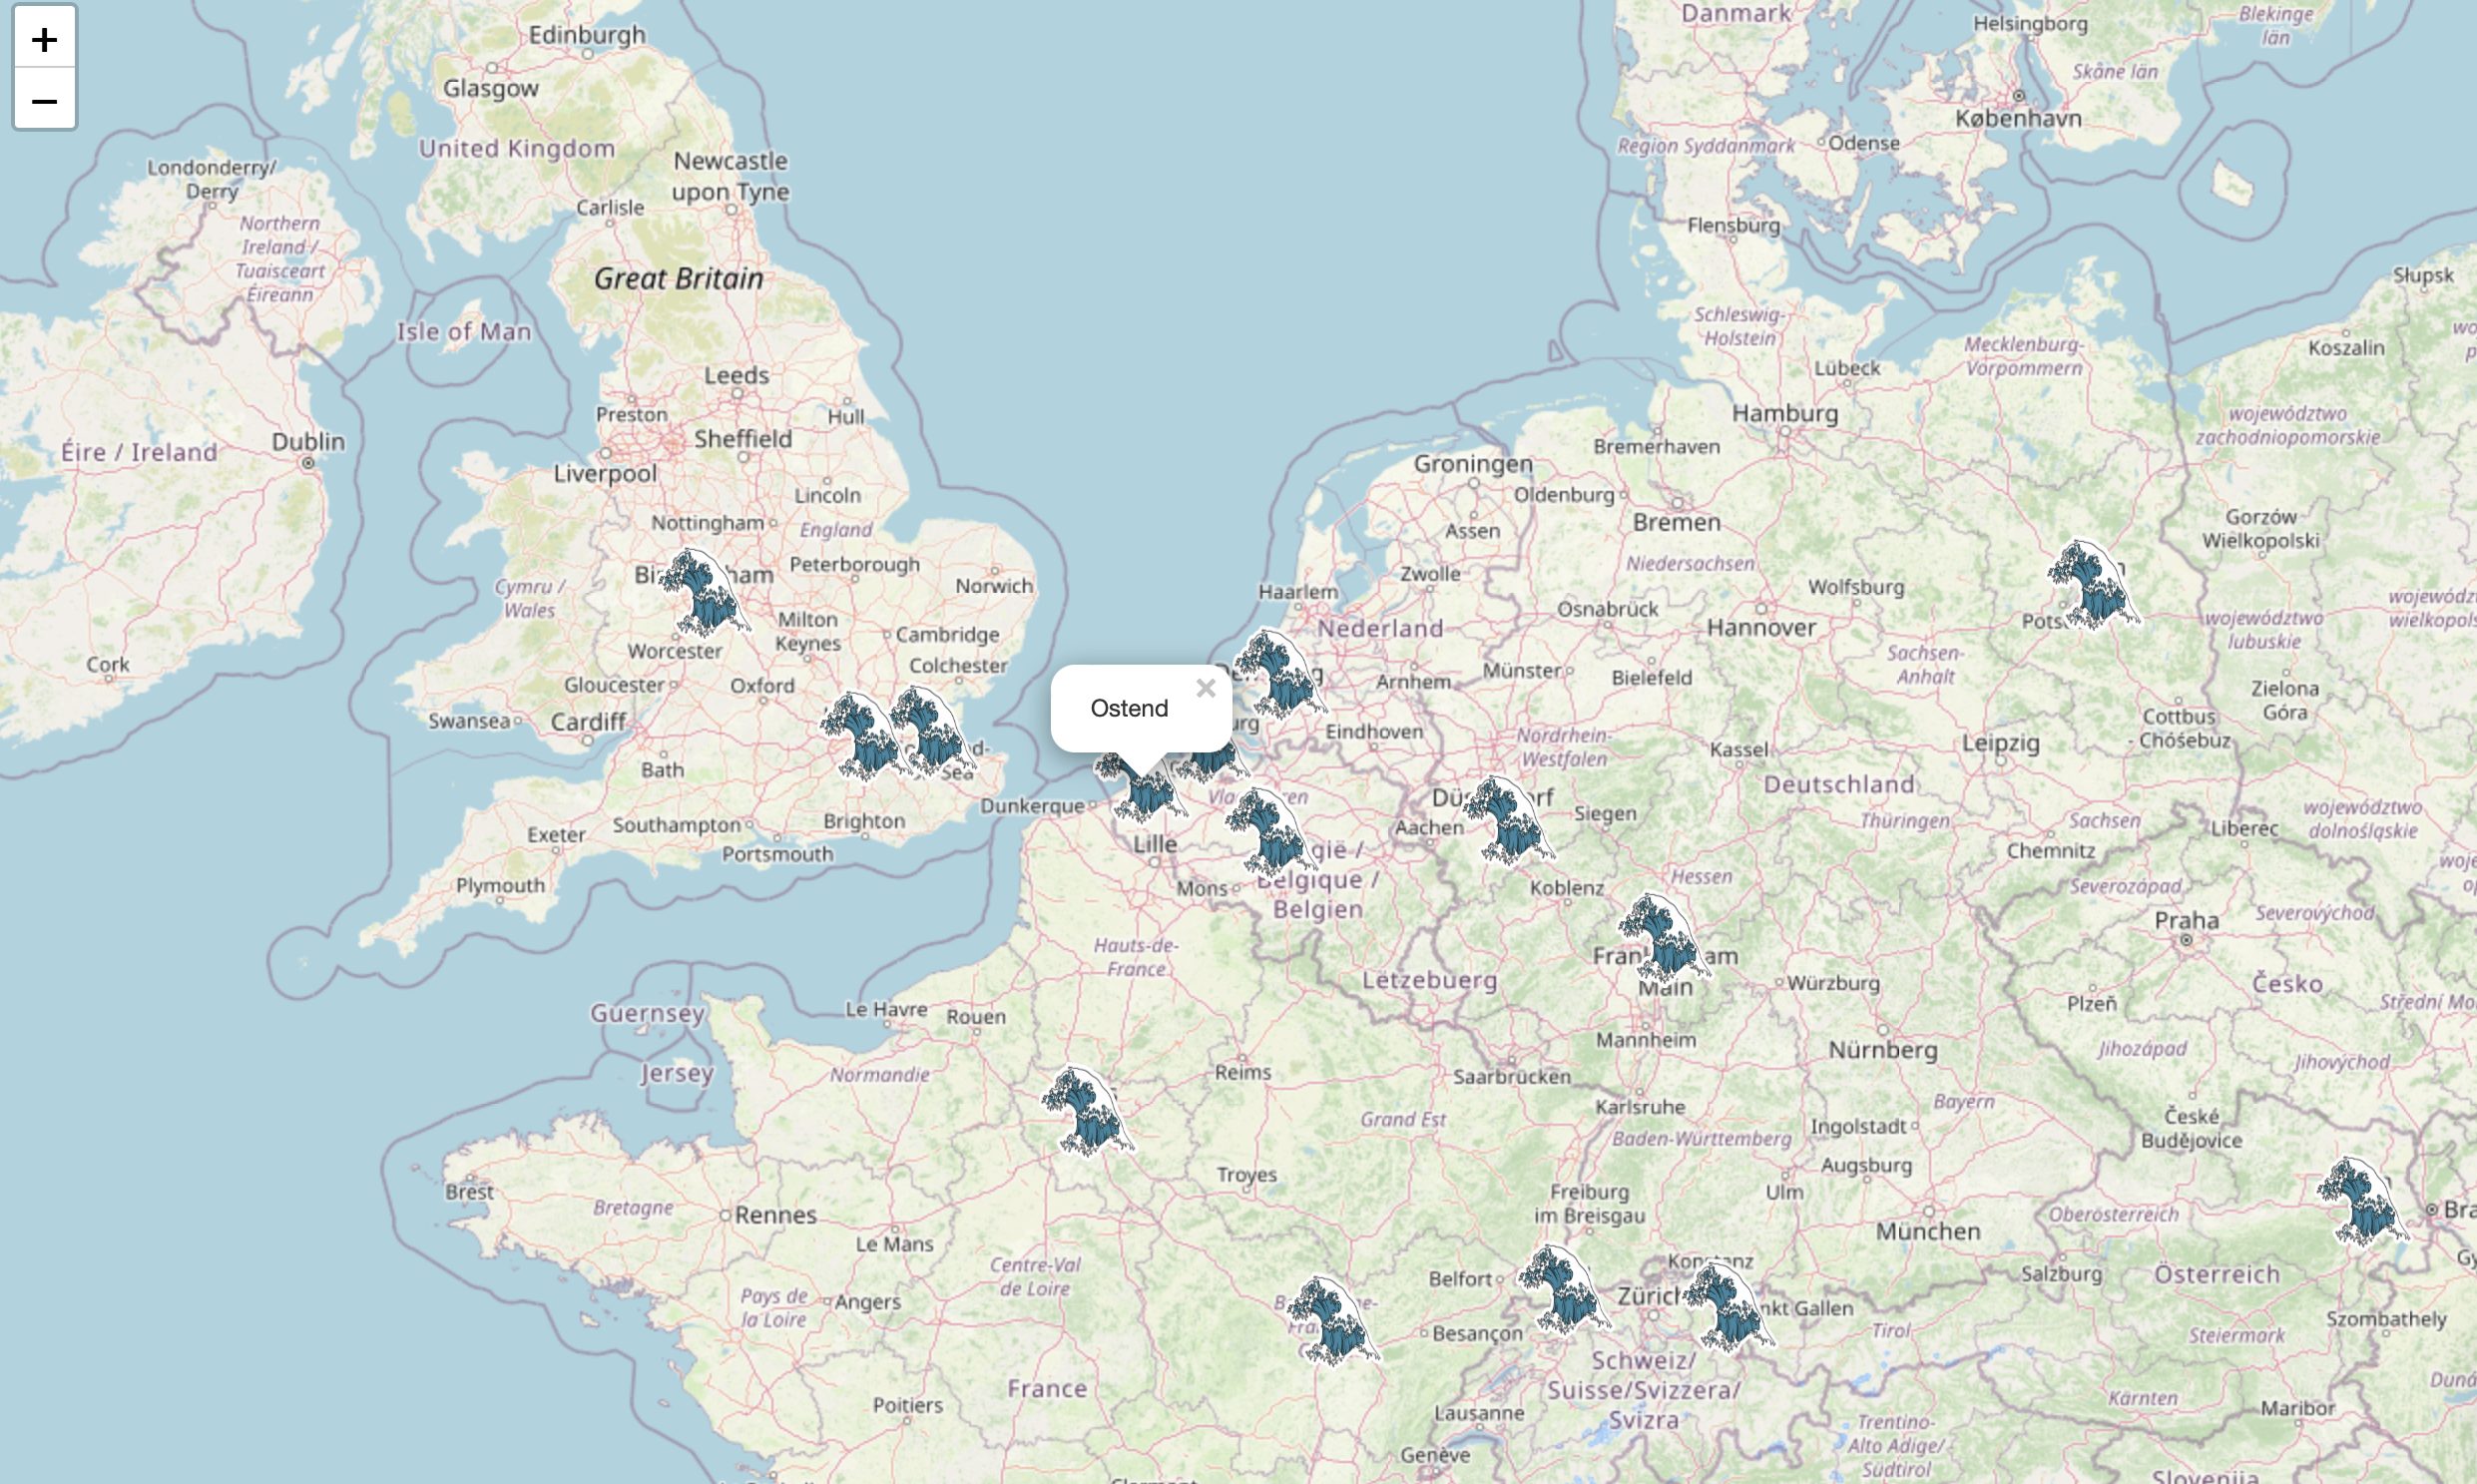
\includegraphics[width=0.5\linewidth]{Screenshot 2023-06-15 at 11.17.19.png}
    \caption{Enter Caption}
    \label{fig:enter-label}
\end{figure}
mutual\\

\begin{figure}
    \centering
    \includegraphics[width=1\linewidth]{Screenshot 2023-06-14 at 23.48.44.png}
    \caption{Enter Caption}
    \label{fig:enter-label}
\end{figure}
\begin{figure}
    \centering
    \includegraphics[width=1\linewidth]{KSqQE 2.png}
    \caption{Enter Caption}
    \label{fig:enter-label}
\end{figure}
\begin{figure}
    \centering
    \includegraphics[width=1\linewidth]{Screenshot 2023-06-15 at 00.41.16.png}
    \caption{Enter Caption}
    \label{fig:enter-label}
\end{figure}


\begin{figure}
    \centering
    \includegraphics[width=1\linewidth]{sea ocean separate.png}
    \caption{Enter Caption}
    \label{fig:enter-label}
\end{figure}
\begin{figure}
    \centering
    \includegraphics[width=1\linewidth]{sea ocean scaled.png}
    \caption{Enter Caption}
    \label{fig:enter-label}
\end{figur

\begin{figure}
    \centering
    \includegraphics[width=1\linewidth]{Screenshot 2023-06-15 at 00.40.59.png}
    \caption{Enter Caption}
    \label{fig:enter-label}
\end{figure}
\begin{figure}
    \centering
    \includegraphics[width=0.5\linewidth]{ocean + city name.png}
    \caption{Enter Caption}
    \label{fig:enter-label}
\end{figure}

\begin{figure}
    \centering
    \includegraphics[width=1\linewidth]{landlocked countries plus ocean.png}
    \caption{Enter Caption}
    \label{fig:enter-label}
\end{figure}

ostend\\



\begin{figure}
    \centering
    \includegraphics[width=1\linewidth]{bel ostend birth.png}
    \caption{Enter Caption}
    \label{fig:enter-label}
\end{figure}
\begin{figure}
    \centering
    \includegraphics[width=0.5\linewidth]{Screenshot 2023-06-15 at 00.39.34.png}
    \caption{Enter Caption}
    \label{fig:enter-label}
\end{figure}

istanbul\\

\begin{figure}
    \centering
    \includegraphics[width=0.5\linewidth]{Screenshot 2023-06-15 at 00.52-1 (dragged).tiff}
    \caption{Enter Caption}
    \label{fig:enter-label}
\end{figure}

\begin{figure}
    \centering
    \includegraphics[width=0.5\linewidth]{istanbul bi birth plavces.png}
    \caption{Enter Caption}
    \label{fig:enter-label}
\end{figure}

\begin{figure}
    \centering
    \includegraphics[width=0.5\linewidth]{Screenshot 2023-06-15 at 00.40.29.png}
    \caption{Enter Caption}
    \label{fig:enter-label}
\end{figure}
\begin{figure}
    \centering
    \includegraphics[width=0.5\linewidth]{istanbul whole world scaled.png}
    \caption{Enter Caption}
    \label{fig:enter-label}
\end{figure}
\begin{figure}
    \centering
    \includegraphics[width=0.5\linewidth]{fend .png}
    \caption{Enter Caption}
    \label{fig:enter-label}
\end{figure}
\begin{figure}
    \centering
    \includegraphics[width=1\linewidth]{Screenshot 2023-06-14 at 19.00.35.png}
    \caption{Enter Caption}
    \label{fig:enter-label}
\end{figure}
\chapter{Conclusions, Limites et Perspectives}

\section{Questionnements méthodologiques}

\section{Perspectives}

\section{Conclusions générales}

\chapter{Bibliographie}

\nocite{Pifsterer, U. (2018) Big Bang Art History, International Journal for Digital Art History, no. 3 (juillet)}
\nocite{Blum, H. (2010). The prospect of Oceanic Studies. PMLA/Publications of the Modern Language Association of America, 125(3), 670-677. https://doi.org/10.1632/pmla.2010.125.3.670 
}
\nocite{Casati, R., Kulvicki, J., & Zeimbekis, J. (2020). Borgesian maps. Analytic Philosophy, 63(2), 90-98. https://doi.org/10.1111/phib.12204 }
\nocite{Casati, R., Kulvicki, J., & Zeimbekis, J. (2020). Borgesian maps. Analytic Philosophy, 63(2), 90-98. https://doi.org/10.1111/phib.12204}
\nocite{Casati, R., Kulvicki, J., & Zeimbekis, J. (2020). Borgesian maps. Analytic Philosophy, 63(2), 90-98. https://doi.org/10.1111/phib.12204 }
\nocite{Clarke, D. J. (2010). Water and art: A Cross Cultural Study of water as subject and medium in modern and contemporary artistic practice. Reaktion Books}
\nocite{Doyle, A. C. (1992). The Maracot deep. Tokyo Sogensha.}
\nocite{Dupont, S. (2017). I am the ocean - arts and sciences to move from ocean literacy to passion for the ocean. Journal of the Marine Biological Association of the United Kingdom, 97(6), 1211-1213. https://doi.org/10.1017/s0025315417000376 }
\nocite{Fluence, T. E. (2014). A vocabulary of water: How water in contemporary art materialises the conditions of contemporaneity. University of Melbourne. }
\nocite{Glissant, É., Nathanaël, & Malena, A. (2018). Poetic intention. Nightboat Books. }
\nocite{Ramírez-Valdivia, M. T. (2017). Memory, Heritage, and Art Production: The Jesús Ramos Frías Art Documentation Center and the Information System on Art Practice in San Luis Potosí. Art Documentation: Journal of the Art Libraries Society of North America, 36(2), 211-221.}
\nocite{Sheehan, T., Smith, M. A., Gant, C., & Jordanous, A. (2019). Meta-Curating: Online Exhibitions Questioning Curatorial Practices in the Postdigital Age. Leonardo, 52(1), 41-47. doi: 10.1162/LEON_a_01254}
\nocite{Wasielewski, A., & Dahlgren, A. (2019). Mining Art History: Bulk Converting Nonstandard PDFs to Text to Determine the Frequency of Citations and Key Terms in Humanities Articles. The Journal of Open Humanities Data, 5(1), 6. doi: 10.5334/johd.23
}
\nocite{Fraiberger, S. P., Sinatra, R., Resch, M., Riedl, C., & Barabási, A. L. (2018). Quantifying reputation and success in art. Science, 362(6416), 825-829. doi: 10.1126/science.aau7224
}
\nocite{Crockett, D. (2019). IVPY: Iconographic Visualization inside Computational Notebooks. Code4Lib Journal, (44). Retrieved from https://journal.code4lib.org/articles/14646}

\nocite{Mercuriali, G. (2018). Digital Art History and the Computational Imagination. International Journal for Digital Art History, 2, 1-19. Retrieved from https://journals.ub.uni-heidelberg.de/index.php/dah/article/download/52660/46328
}

\nocite{Bentkowska-Kafel, A. (2016). Debating Digital Art History. Visual Resources, 32(1-2), 13-39. doi: 10.1080/01973762.2016.1141458}

\nocite{Steinberg, P. E. (2013). Of other seas: Metaphors and materialities in maritime regions. Atlantic Studies, 10(2), 156-169. https://doi.org/10.1080/14788810.2013.785192 }

\nocite{Peters, K., & Steinberg, P. (2019). The ocean in excess: Towards a more-than-wet ontology. Dialogues in Human Geography, 9(3), 293-307. https://doi.org/10.1177/2043820619872886 
}

\nocite{Osborne, P. (2013). Anywhere or not at all: Philosophy of contemporary art. Verso. }
\nocite{Morton, T. (2021). Hyperobjects philosophy and ecology after the end of the world. University of Minnesota Press. }
\nocite{Morton, T. (2018). Dark ecology: For a logic of future coexistence. Columbia University Press. }
\nocite{London, J., & Oblonskai͡a R. E. (2020). Martin Iden. Rosmėn. }
\nocite{Lem, S., Jasienko, J.-M., & Lem, S. (2021). Solaris. Actes Sud. }
\nocite{Katz, E., Light, A., & Rothenberg, D. (2000). Beneath the surface: Critical essays in the philosophy of Deep Ecology. The MIT Press. }
\nocite{Doulkaridou, E. (2018). Reframing Art History. Mit Press.}
\nocite{Terras, M., Nyhan, J., & Vanhoutte, E. (Eds.). (2018). The Routledge Companion to Digital Humanities and Art History. Routledge.}
\nocite{Bönisch, D., Loos, L., & de Wilde, M. (2018). The Curator's Machine: Clustering of Museum Collection Data through Annotation of Hidden Connection Patterns between Artworks. In Balancing between Trade and Ideology (pp. 311-320). Springer.
}
\nocite{Wasielewski, A. (2019). The Growing Pains of Digital Art History: Issues for the Study of Art Using Computational Methods. In The Shape of Data in Digital Humanities (pp. 275-298). Routledge.
}
\nocite{Velthuis, O., & Baia Curioni, S. (2018). The history of art markets: methodological considerations from art history and cultural economics. Journal of Cultural Economics, 42(2), 161-178.}
\nocite{Drucker, J. (2013). The shape of data in the digital humanities. In Debates in the Digital Humanities (pp. 229-246). University of Minnesota Press.}
\nocite{Bal, M., &amp; Bryce, N. (2001). Looking in: The art of viewing. Routledge.
}
\nocite{Bauman, Z. (2017). Liquid times: Living in an age of uncertainty. Polity Press.
}
\nocite{Blum, H. (2010). The prospect of Oceanic Studies. PMLA/Publications of the Modern Language Association of America, 125(3), 670–677. doi: 10.1632/pmla.2010.125.3.670
}
\nocite{Boero, N., & Mason, K. (Eds.). (2021). The Oxford Handbook of the sociology of body and embodiment. Oxford University Press.}
\nocite{Burdick, A., Drucker, J., Lunenfeld, P., Presner, T. S., & Schnapp, J. T. (2012). Digital_Humanities. The MIT Press.}
\nocite{Burrough, P. A., & Frank, A. U. (1996). Geographic objects with indeterminate boundaries. Taylor & Francis.}
\nocite{Buskirk, M. (2005). The contingent object of Contemporary Art. MIT.
}
\nocite{Clarke, D. (2010). Water and art: A cross-cultural study of water as subject and medium in modern and contemporary artistic practice. Reaktion Books.}
\nocite{Cusack, D. R. (2016). Art and identity at the water's edge. Routledge.
}
\nocite{Dupont, S. (2017). I am the ocean – arts and sciences to move from ocean literacy to passion for the ocean. Journal of the Marine Biological Association of the United Kingdom, 97(6), 1211–1213. doi: 10.1017/s0025315417000376}
\nocite{Fluence, T. E. (2014). A vocabulary of water: How water in contemporary art materialises the conditions of contemporaneity. University of Melbourne.
}
\nocite{Gardiner, E., & Musto, R. G. (2015). The Digital Humanities: A Primer for Students and Scholars. Cambridge University Press.}
\nocite{Helmreich, S., Roosth, S., & Friedner, M. (2016). Sounding the limits of life: Essays in the anthropology of biology and beyond. Princeton University Press.}
\nocite{Holtaway, J. (2021). World-forming and Contemporary Art. Routledge.}
\nocite{Isto, R. (2015). Organic (UN)ground in the time of biopower and hyperobjects: Conceptualizing global posthumanism in the art of Xu Bing and Gu Wenda. Journal of Contemporary Chinese Art, 2(2), 195–215. doi: 10.1386/jcca.2.2-3.195_1}
\nocite{Johnson, P. (2020). Art that lives and breathes: Conserving creatures in contemporary art. Journal of the American Institute for Conservation, 60(2-3), 175–185. doi: 10.1080/01971360.2020.1790093}
\nocite{Latour, B., & Porter, C. (1998). We have never been modern. Harvard University Press.
}
\nocite{Lestel, D. (2018). Dissolving Nature in Culture. The Philosophical Ethology of Dominique Lestel. doi: 10.4324/9781315158631-8}
\nocite{Magnason, A. (2022). On Time and Water. Open Letter Press.}
\nocite{Manning, C. D., & Schutze, H. (1999). Foundations of Statistical Natural Language Processing. MIT.
}
\nocite{Manovich, L. (2001). The Language of New Media. MIT Press.}
\nocite{Manovich, L. (2020). Cultural Analytics. The MIT Press.}

\nocite{Meillassoux, Q., Meillassoux, C. (2011). Time without Becoming. Mimesis Edizioni.}
\nocite{Meillassoux, Q., Brassier, R., & Badiou, A. (2008). After Finitude: An Essay on the Necessity of Contingency. Bloomsbury Academic.}
\nocite{Meyer, G. (2020). Ocean Inspired Mathematical Art. Journal of Mathematics and the Arts, 14(1-2), 108–110. doi: 10.1080/17513472.2020.1751576}

\nocite{Morton, T. (2007). Ecology without Nature: Rethinking Environmental Aesthetics. Harvard University Press.
}
\nocite{Morton, T. (2013). Hyperobjects: Philosophy and Ecology after the End of the World. University of Minnesota Press.
}
\nocite{Moser, K. A., & Sukla, A. C. (2020). Imagination and Art: Explorations in Contemporary Theory. Brill Rodopi.}
\nocite{Neimanis, A. (2017). Bodies of Water: Posthuman Feminist Phenomenology. Bloomsbury.}
\nocite{Neset, A. (2009). Arcadian Waters and Wanton Seas: The Iconology of Waterscapes in Nineteenth-Century Transatlantic Culture. Lang.}
\nocite{Osborne, P. (2013). Anywhere or not at all: Philosophy of contemporary art. Verso.}
\nocite{Oyarzun, V. E. (2020). Avenging nature: The role of nature in modern and contemporary art and literature. Lexington Books, an imprint of The Rowman &amp; Littlefield Publishing Group, Inc.}
\nocite{Roberts, C. (2009). The unnatural history of the sea. Island Press.}

\nocite{Ross, C. (2014). The past is the present, it's the future too: The temporal turn in contemporary art. Bloomsbury.}

\nocite{Smith, T., Enwezor, O., &amp; Condee, N. (2008). Antinomies of art and culture: Modernity, postmodernity, contemporaneity. Duke University Press.}
\nocite{Steinberg, P. E. (2001). The social construction of the Ocean. Cambridge University Press.}
\nocite{Steinberg, P. E. (2013). Of other seas: Metaphors and materialities in maritime regions. Atlantic Studies, 10(2), 156–169. doi: 10.1080/14788810.2013.785192}
\nocite{Vignemont, F. de. (2020). Mind the body: An exploration of bodily self-awareness. Oxford University Press.}
\nocite{Wen, X., &amp; White, P. (2020). The role of landscape art in cultural and national identity: Chinese and European comparisons. Sustainability, 12(13), 5472. doi: 10.3390/su12135472}
\nocite{Zhai, C. X., &amp; Massung, S. (2016). Text Data Management and Analysis: A Practical Introduction to Information Retrieval and Text Mining. Association for Computing Machinery.}

\newpage
\printbibliography[title=Bibliographie]
\listoffigures[title=Les figures]
\end{document}  author={Casati, R. and Kulvicki, J. and Zeimbekis, J.},